\documentclass{article}
\usepackage[utf8]{inputenc}
\usepackage{listings}
\usepackage{float}
\usepackage{natbib}
\usepackage{graphicx}
\usepackage{amssymb}
\usepackage{amsmath}
\usepackage{amsthm}
\usepackage{mathtools}
\usepackage{listings}
\usepackage{color}
\usepackage{hyperref}
\usepackage{ amssymb }
\usepackage{musicography}
\usepackage{physics}
\NeedsTeXFormat{LaTeX2e}
\ProvidesPackage{quiver}[2020/11/27 quiver]
\newtheorem{theorem}{Theorem}[section]
\newtheorem{corollary}{Corollary}[theorem]
\newtheorem{lemma}[theorem]{Lemma}

% `tikz-cd` is necessary to draw commutative diagrams.
\RequirePackage{tikz-cd}
% `calc` is necessary to draw curved arrows.
\usetikzlibrary{calc}
% `pathmorphing` is necessary to draw squiggly arrows.
\usetikzlibrary{decorations.pathmorphing}

\definecolor{dkgreen}{rgb}{0,0.6,0}
\definecolor{gray}{rgb}{0.5,0.5,0.5}
\definecolor{mauve}{rgb}{0.58,0,0.82}

\tikzset{curve/.style={settings={#1},to path={(\tikztostart)
    .. controls ($(\tikztostart)!\pv{pos}!(\tikztotarget)!\pv{height}!270:(\tikztotarget)$)
    and ($(\tikztostart)!1-\pv{pos}!(\tikztotarget)!\pv{height}!270:(\tikztotarget)$)
    .. (\tikztotarget)\tikztonodes}},
    settings/.code={\tikzset{quiver/.cd,#1}
        \def\pv##1{\pgfkeysvalueof{/tikz/quiver/##1}}},
    quiver/.cd,pos/.initial=0.35,height/.initial=0}

% TikZ arrowhead/tail styles.
\tikzset{tail reversed/.code={\pgfsetarrowsstart{tikzcd to}}}
\tikzset{2tail/.code={\pgfsetarrowsstart{Implies[reversed]}}}
\tikzset{2tail reversed/.code={\pgfsetarrowsstart{Implies}}}

\lstset{frame=tb,
  language=Scala,
  aboveskip=3mm,
  belowskip=3mm,
  showstringspaces=false,
  columns=flexible,
  basicstyle={\small\ttfamily},
  numbers=none,
  numberstyle=\tiny\color{gray},
  keywordstyle=\color{blue},
  commentstyle=\color{dkgreen},
  stringstyle=\color{mauve},
  breaklines=true,
  breakatwhitespace=true,
  tabsize=3
}
\newcommand{\colim}{\operatorname{colim}}

\newcommand\rightthreearrow{%
        \mathrel{\vcenter{\mathsurround0pt
                \ialign{##\crcr
                        \noalign{\nointerlineskip}$\rightarrow$\crcr
                        \noalign{\nointerlineskip}$\rightarrow$\crcr
                        \noalign{\nointerlineskip}$\rightarrow$\crcr
                }%
        }}%
}

\newcommand\righttwoarrow{%
        \mathrel{\vcenter{\mathsurround0pt
                \ialign{##\crcr
                        \noalign{\nointerlineskip}$\rightarrow$\crcr
                        \noalign{\nointerlineskip}$\rightarrow$\crcr
                }%
        }}%
}

\graphicspath{ {./images/} }

\title{Generative Calculus and the economic theory of Generativity}
\author{Wyatt L. Meldman-Floch}
\date{December 21, 2020}
\setlength{\parskip}{1em}

\begin{document}
\maketitle

\begin{abstract}
A new economic system designed to maximize the utility through autonomous infrastructure is presented.
A global interpreter for interaction and deployment of this infrastructure as well as an associated programming language specification is constructed.
These constructions are then used to define the "Economic Engine" and via the Second Law of Thermodynamics prove that the stability of the economy is proportional to the efficiency and volume of resources provided to host it.

\end{abstract}

\tableofcontents

\setcounter{secnumdepth}{0}



\section{Acknowledgments}
In loving memory of Leonard Meldman and Jim Valentine.

\section{The Generative Calculus}
The context within which our model exists are recent advancements in distributed ledger technology, namely Cryptocurrencies.
Traditionally a Cryptocurrency is just a speculative asset like a security that also has some real world technological use case, but in general the value of the currency is tied to speculation and not to any verifiable measure of utility.
The following is a reformulation of Cryptocurrencies as a commodification of the utility provided by a distributed consensus protocol.

The recent advancements in distributed ledger technology alluded to revolve around scalability.
Consensus protocols with a linear/block data model such as Bitcoin and Ethereum are fundamentally incompatible with the advent of microservice architectures which define the paradigm of network architecture for large scale data processing systems. 
In most cases they are distributed systems that operate in serial, which is antithetical to the concurrent underpinnings of distributed systems; horizontal scalability and efficient data locality. 
In order to apply the utility of a distributed consensus protocol to large scale data processing systems, they must be fully compatible with dynamic scaling and deployment features such as elastic deployment and dynamic partitioning.
As the backbone to Cruyptocurrencies the economic incentive to provide computational resources, a key requirement is the ability for their validator rewards models to dynamically adjust in tandem with network organization.
An emerging class of consensus protocols overcome these limitations with a nonlinear data model known as a directed acyclic graph (DAG.)
HGTP, the core technology developed from the Cohomology Theory of Blockchain Technology and backbone of the HyperGraph Network will be referenced periodically throughout the rest of this work as a real world technology that implement these principles.

The following constructions form a calculus, namely the Calculus of Generations, which apply to dynamical systems of generative effects. 
As has been shown in previous works, consensus protocols are equivalently described via the category of chain complexes which map directly to generative effects. Generative Calculus allows for geometric representation and analysis of quantities defined by generative effects, which are then used in the next section to define a macroeconomic theory of market stability for Cryptocurrencies that is an extension of The Economic Theory of General Equilibrium.

\subsection{The Category of Differentiable Consensus Protocols}
First, let's construct a universal context to axiomatize the mechanics of distributed consensus protocols by employing the principle construction of Blockchain Cohomology: the Poincare Complex.
The Poincare Complex is a generic combinatorial model for consensus systems, where network state is described in terms of simplicial geometry and transitions are defined in terms of a discrete gradient. 
Its main advantage is that it symbolically represents the requirements for consensus protocols to be defined recursively, forming a network with hierarchical mesh topology\footnote{KFUPM chapter on designing a network topology, see chapter 5\\ \url{http://faculty.kfupm.edu.sa/coe/marwan/richfiles/Designing\%20a\%20Network\%20Topology.pdf}}, which is optimal for a highly available network of heterogeneous devices in its definition as a Functorial Operator.
The Poincare Complex was constructed using the language of algebraic topology because it simplifies correctness proofs into constructivist logic (proof by construction) by reducing the context of the problem to spaces.
However, the converse is true in classifying instances of a Poincare Complex.
Fortunately, due to the focus on homotopy types in the construction of the Poincare Complex, there is an equivalent construction by means of a category, which will soon be defined as the Category of Consensus Protocols.
Category theory is helpful in that it organizes, frames, and contextualizes information so it can be managed easier, and one can often prove statements in the abstract setting of categories and functors and then apply them to particular situations.
The Category of Consensus Protocols can then be extened to create a "universal construction" that allows for mappings across or compositions of Consensus Protocols that retain the same guarantees as the starting Consensus Protocols, by means of defining a particular functor.
Functors are mappings between categories which are used to define this notion of equivalence. 
Let's use this functorial operator to construct a proper category and use the functors of this category to define a universal context for Consensus Protocols.

Consider the Poincare Complex
\begin{equation}
\Omega^T_\Gamma: 0 \xleftrightarrow{\partial} \Omega^{T^*}_{\Gamma^*}(\epsilon) \xleftrightarrow{\partial} \Omega^T_\Gamma (\epsilon(P_0)) \dots \Omega^T_\Gamma (\epsilon(P_\pi))
\end{equation}
where $\Omega^T_\Gamma$ is a functor obeying the laws of the Protocol Manifold\footnote{Meldman-Floch, Wyatt, ``Blockchain Cohomology: Sec 23' \\ http://ceur-ws.org/Vol-2478/paper2.pdf} (or the data structure of State Data governed by the protocol), Protocol Topology\footnote{Meldman-Floch, Wyatt, ``Blockchain Cohomology: Sec 2'' \\ http://ceur-ws.org/Vol-2478/paper2.pdf} (the organization of the physical machines themselves) and functoral group homomorphisms gHylo, a generalization of Hylomorphism that allows any combination of refolds out of comonadic recursion schemes\footnote{Patrick Thomson, ``recursion-schemes-part-6' \\ https://blog.sumtypeofway.com/posts/recursion-schemes-part-6.html}. These refolds are all defined as a combination of catamorphism and anamorphism where the f-algebra and dual f-coalgebra which maintain Poincare duality of the protocol manifold up to $\pi$ isomorphism. 
In terms of $\Sigma$ and $\epsilon$, where the functor $\Sigma$ is a valid f-algebra and sheaf $\epsilon$ a co-algebra, this combination forms the "Gather Apply Scatter."

A Hylomorphism or "Gather Apply"
\begin{equation}
\epsilon \leftarrow P \times \Sigma: \Omega^T(\epsilon, P)
\end{equation}
and Metamorphism which is a valid refold or a "Scatter"
\begin{equation}
\Omega_\Gamma(P, \epsilon):\Gamma_\Sigma \times \epsilon \rightarrow P
\end{equation} 
are constructions that encapsulate the two directions of the distributive laws required for a commutative monad\footnote{gelisam, "use Gather/Scatter instead of distributive laws", \\ https://github.com/ekmett/recursion-schemes/pull/51} as is known in functional programming; further examples of gHylo constructions can be found in Tessellation\footnote{buckysballs, "name of pr", \\ https://github.com/tessellation/}.
Note that any refold satisfying duality of recursion is a valid Scatter.

The original construction of the Poincare Complex used the sheaf cohomology of synthetic differential geometry to create a topological space classified by homotopy equivalence between "state spaces", where homotopy is defined by functor algebra invariants. Specifically the most basic invariants are the homotopy group $\pi$, the homology group $\Omega_\Gamma$ and cohomology group $\Omega^T$.  
These invariants assign a group structure to a space with graded abelian algebra.
But they also define a homomorphism (a map of groups) to each map of spaces. 
This feature allows us to transfer comparisons between spaces (the role of maps in topology) to comparisons between groups.

\begin{theorem}
$\pi$, $\Omega_\Gamma$ and $\Omega^T$ are functors from the category of topological spaces to the category of groups
\end{theorem}

\begin{proof}
It is equivalent to say that $\pi$, $\Omega_\Gamma$ and $\Omega^T$ are functors from the category of topological spaces to the category of groups, because for each $k$ the following commutative diagrams commute:

Composition of $\Omega_\Gamma$
% https://q.uiver.app/?q=WzAsNixbMCwwLCJYIl0sWzIsMCwiWSJdLFsyLDIsIlxccGlfayhZKSJdLFswLDIsIlxccGlfayhYKSJdLFsxLDJdLFszLDIsIlxcYnVsbGV0Il0sWzAsMywiXFxwaV9rIiwyXSxbMywyLCJcXHBpX2soZikiXSxbMCwxLCJmIl0sWzEsMiwiXFxwaV9rKGYpIl1d
\[\begin{tikzcd}
	{X} && {Y} \\
	\\
	{\pi_k(X)} & {} & {\pi_k(Y)}
	\arrow["{\pi_k}"', from=1-1, to=3-1]
	\arrow["{\pi_k(f)}", from=3-1, to=3-3]
	\arrow["{f}", from=1-1, to=1-3]
	\arrow["{\pi_k(f)}", from=1-3, to=3-3]
\end{tikzcd}\]

Composition of $\Omega^T$
% https://q.uiver.app/?q=WzAsNSxbMCwwLCJYIl0sWzIsMCwiWSJdLFsyLDIsIlxcT21lZ2FeayhZKSJdLFswLDIsIlxcT21lZ2FeayhYKSJdLFsxLDJdLFswLDMsIlxcT21lZ2FeayIsMl0sWzMsMiwiXFxPbWVnYV5rKGYpIiwwLHsic3R5bGUiOnsidGFpbCI6eyJuYW1lIjoiYXJyb3doZWFkIn0sImhlYWQiOnsibmFtZSI6Im5vbmUifX19XSxbMCwxLCJmIl0sWzEsMiwiXFxPbWVnYV5rIl1d
\[\begin{tikzcd}
	{X} && {Y} \\
	\\
	{\Omega^k(X)} & {} & {\Omega^k(Y)}
	\arrow["{\Omega^k}"', from=1-1, to=3-1]
	\arrow["{\Omega^k(f)}", from=3-1, to=3-3, tail reversed, no head]
	\arrow["{f}", from=1-1, to=1-3]
	\arrow["{\Omega^k}", from=1-3, to=3-3]
\end{tikzcd}\]

Specifically a Category C consists of 

$\bullet$ Axiom A) A class of objects $Ob(C)$

$\bullet$ Axiom B) For any two objects $X$ and $Y$ $\in Ob(C)$, a class of morphisms (or equivalently maps/arrows) $Hom_C(X,Y)$ for some $ f: X \rightarrow Y$ and for an element $f \in Hom_C(X,Y)$ such that there is a composition function $Hom_C(X,Y) \times Hom_C(Y, Z) \rightarrow Hom_C(X, Z)$ $=>$ $(f, g) \rightarrow g \circ f$ that satisfies the usual associativity and identity axioms.

\begin{lemma}
The Category of Consensus Protocols is a Category of sheaves.
\end{lemma}

\begin{proof}
Define the Category of Consensus Reaching Systems as a presheaf category
\begin{equation}
\mathcal{C}: \{Obj(\mathcal{C}): \{\Omega^T_\Gamma \} | \rightarrow:  \Omega^T \circ \Omega_\Gamma \}
\end{equation}
\end{proof}

If follows by construction that arrows $\partial$ satisfy Axiom B via the compositions proofs of $ \Omega^T$ and $\Omega_\Gamma$ and our object $\Omega^T_\Gamma$ satisfied Axiom A by definition.

Given two objects $P, Q \in$ $ \mathcal{C}$ the Poincare Protocol a morphism $\alpha: P \rightarrow Q$ between them is a natural transformation of functors such that 
% https://q.uiver.app/?q=WzAsNCxbMCwwLCJcXG1hdGhjYWx7Q30iXSxbMiwwLCJIeXAgIl0sWzEsMCwiXFxkb3duYXJyb3cgXFxwYXJ0aWFsIl0sWzMsMCwiU2V0Il0sWzAsMSwiUSIsMix7ImN1cnZlIjo1fV0sWzAsMSwiUCIsMCx7ImN1cnZlIjotNX1dLFsxLDNdXQ==
\[\begin{tikzcd}
	{\mathcal{C}} & {\downarrow \partial} & {Hyp } & {Set}
	\arrow["{Q}"', from=1-1, to=1-3, curve={height=30pt}]
	\arrow["{P}", from=1-1, to=1-3, curve={height=-30pt}]
	\arrow[from=1-3, to=1-4]
\end{tikzcd}\]
via the enrichment of geometric cw-complexes has strict ordering enforced by deRham cohomology of $\Omega^T_\Gamma$ objects, satisfying the presheaf condition due to the existence of forgetful functors into the category of hypergraphs for all deRham complexes. 
\end{proof}

\subsubsection{The Consensus Topos}
The Poincare Protocol was defined in terms of a special topological object called a sheaf $\epsilon$ which is an object that encapsulates action within a space. 
The idea is similar to how basis are managed in ordinary vector calculus but extended to abstract spaces.
In differential geometry sites, (one element of the sheaf object), are "stitched together" to form a domain upon which differential forms, which lead to proper calculus, can be conducted; as will be demonstrated later, this is core to the derivation of the utility function.
Formulating in terms of sheaves yields the ability to construct a topos, a special kind of category for "behavior types" whose objects are configuration state changes through time.
This allows the verification of processes and even quantification of their safety, which is the goal of wider field of Complex Systems of Systems Theory\footnote{Spivek et. al., "Abstraction, Composition and Contracts:A Sheaf Theoretic Approachr", \\ https://arxiv.org/pdf/1802.03080.pdf}.
Further research shows that applications of Blockchain technology and even the teminology (Contracts etc.) are in essence just extensions of logic proofs defined in terms of the intuitionistic logic of a topos.
Let's construct the topos of Poincare Protocols so it can be used as a context for the rest of the paper.

\begin{theorem}
A Category of Sheaves is a topos
\end{theorem}

\begin{proof}
A Category of Sheaves is a topos, if the following conditions are met:

$\bullet$ Axiom C) The sheaf condition of a presheaf $\epsilon$ is satisfied\footnote{Spivek et. al., Definition 7.35, "Abstraction, Composition and Contracts:A Sheaf Theoretic Approachr", \\ https://arxiv.org/pdf/1802.03080.pdf}, namely there exists a matching family of p-sections over a "covering" or collection of open sets contained within an object, such that for each section within the presheaf, the matching families are equivalent up to Homotopy. If there exists a unique gluing for every matching family we say that P satisfies the sheaf condition for the cover.

Proof of Axiom C: Recall the de Rham complex of the definition of the Poincare Protocol
\begin{equation}
\Gamma_X(S^*):  0 \xrightarrow{~} \Gamma_X(\epsilon) \xrightarrow{d^0} \Gamma_X(S^0) \xrightarrow{d^1} \dots
\end{equation}
a topology $X$ defined by an acyclic resolution the "block-sheaf" $\epsilon$ which is an A-module sheaf $\epsilon(X)$ over topological space $X$, can be described by global sections $\Gamma_X(\epsilon) \equiv \Gamma (X, \epsilon)$
\begin{equation}
H_n(X, \epsilon) := R^n(\Gamma(C,\epsilon) := H^n[\Gamma(C, S^*)] := ker\Gamma_X(d^n)/im\Gamma_X(d^{n-1})
\end{equation}
where $R^n\Gamma$ is the right derived functor of the global section functor $\Gamma_x(.) \equiv \Gamma(X,.)$ where $R^n$ is equivalent to the $i^{th}$ linear ringed subspace above. 
Given two topological spaces, $X$ and $Y$ $\in \mathcal{C}$, an open subset $Op \subseteq P(X) | P(X) = \{ U \subseteq X\}$ and $\Gamma: Op \rightarrow Hyp \rightarrow Set$, via the singular homology of chain complexes carried by the protocol topology $\Sigma$\footnote{eq 8, B Cohomology}, the global sections for each topology are unique up to homotopy, which means that right-derived functor $H_n$ defines the $\mathbb{A}$-resolution of a sheaf $\epsilon$ with unique covering for all $\Gamma$, which satisfies the sheaf condition.

$\bullet$ Axiom D) There exists a "subobject classifier" $\Omega$ the object of truth values, such that $\Omega$ is the presheaf that assigns $U \in Obj$ the set of open subsets of $U$: 
\begin{equation}
\Omega(U) := \{ U' \in Obj | U' \subseteq U\}
\end{equation}

Proof of Axiom D: this is trivial, it is the presheaf of the linear subspaces of the sheaf cohomology of the de Rham complex used in defining $\epsilon$.
\end{proof}

We now have the Consensus Topos
\begin{equation}
\mathcal{E} := Shv(\Omega^T_\Gamma, Op)
\end{equation}
which is a sheaf topos of Poincare Protocols.

\subsection{A Day Construction of Generative Effects}
The Consensus Topos is a powerful object in that it can be used to quantify the compatibility of consensus protocols and calculate measures of Consensus Protocol safety by extending the well known Calculus of Functors. 
Calculus of Functors is a theory that aims to “approximate” functors in algebra and topology much like the Taylor polynomials approximate ordinary smooth real or complex-valued functions.
Functors of the Consensus Topos are compatible with the calculus of functors, but in order to incorporate system guarantees, the enrichment of these functors is required for concrete metrics.
This is where Generative Calculus comes in.
Behavioral Types can be quantified and analyzed in terms of Generative Effects, namely by the Generative Calculus which is defined below.

The Generative Calculus is largely an extension and in some ways simplification of the Abelian Functor Calculus, which is the calculus of functors of abelian categories.
The construction of a directional derivative for abelian categories provides an abstract framework that makes certain analogies between classical and functor calculus explicit.
This analogy as will be shown, is necessary to calculate metrics in the consensus topos using de rham cohomology (a measure of how well the fundamental theorem of calculus holds up) to quantify 'lossiness' similar to the theory of error correction codes.
By further reducing the arrows of the category to a day convolution, Generative Calculus calculates safety in terms of manifold deformaions/energy loss or equivalently in the language of fourier transforms, decoherence.
First, let's start from the definition of Abelian Functor Calculus and its associated directional derivative.
Within that context the Generative Calculus will be defined followed by proofs of properties specified.

In order to take advantage of the Abelian Functor Calculus of Bauer et. al. we need show that the ConTop is an appropriate abelian category.
Fortunately, their construction relies on homotopy equivalence which has been previously shown for Poincare Protocols\footnote{Blockchain Cohomology}. 

\begin{lemma}
By identifying a comonad $C_n$ on the category of all functors between a fixed pair of abelian categories, and defining $P_nF$ directly as a resolution of $F$ by this comonad, a Taylor tower of abelian categories is derived.
\end{lemma}

\begin{proof}
For an abelian category $\mathcal{A}$, let $Ch\mathcal{A}$ denote the category of chain complexes on $\mathcal{A}$.
By means of totalization via the methods used by JM2\footnote{[JM2, Lemma 5.7] https://arxiv.org/pdf/1610.01930.pdf} the category of chain complexes can be considered a pseudomonad acting on the large 2-category of abelian categories, arbitrary functors between them and natural transformations.
Consider the quotient monad $Ch(-)$ acting on the 1-category $AbCat$ of abelian categories and isomorphism classes of functors:

$\bullet$ Axiom A) The monad carries an abelian category $\mathcal{A}$ to the category $Ch\mathcal{A}$ of non-negativelygraded chain complexes in $\mathcal{A}$

$\bullet$ Axiom B) The monad carries a functor $F: B \rightarrow A$ to its prolongation $Ch F: Ch B \rightarrow Ch A$. 
By way of the Dold-Kan equivalence between non-negatively graded chain complexes and simplicial objects, the functor $Ch F$is defined to be the composite
\begin{equation}
ChF: Ch\mathcal{B} \xrightarrow{\cong} \mathcal{B}^{\Delta op} \xrightarrow{F_*} \mathcal{A}^{\Delta op} \xrightarrow{\cong} \mathcal{A}
\end{equation}
where the action of $F$ on simplicial objects is by post-composition.

$\bullet$ Axiom C) The components of the unit of the monad are the functors
\begin{equation}
\mathcal{A} \xrightarrow{deg_0} Ch\mathcal{A} 
\end{equation}
hat embed $\mathcal{A}$ as the subcategory of chain complexes concentrated in degree zero.

$\bullet$ Axiom D) If the components of the multiplication of the monad are the functors 
\begin{equation}
ChCH\mathcal{A} \xrightarrow{Tot} Ch\mathcal{A}
\end{equation}
that convert a "double complex" (chain complex of chain complexes, who's squares commute) in $\mathcal{A}$ into a chain complex in $\mathcal{A}$ by forming the "total complex".

\end{proof}

An equivalent monad can be constructed from ConTop.

\begin{theorem}
The Protocol Complex used to construct ConTop can be used to construct a monad $Th(-)$ that is equivalent to $Ch$.
\end{theorem}

\begin{proof}
The Protocol Complex used to construct ConTop can be used to construct a monad $Th(-)$ that has the following properties:

$\bullet$ Axiom A) by eq 11\footnote{Blockchain Cohomology} ConTop's sheaf $\epsilon$ is defined as ’enrichment’ of any cochain A-complex of positive degree/grade,  corresponding  to the A-resolution  of  an  abstract A-module, a non-negatively graded chain complex in $\mathcal{A}$. Thus all functors and thus monads in a Consensus category share the same subobject classifier $\Omega$. Thus any monad in ConTop carries an abelian category given by the A-module into $\mathcal{A}$ to the category $Ch\mathcal{A}$ of non-negatively graded chain complexes in $\mathcal{A}$

$\bullet$ Axiom B) The Protocol Complex (eq 9), chain homotopy for successive functors $\sigma$ are homotopy preserving graded abelian group morphisms with vanishing homology, which by definition satisfy the coherence conditions required by the composite functor $Ch F$ in Axiom B

$\bullet$ Axiom C) This is again shown by chain homotopy of (eq 9) of the Protocol Complex

$\bullet$ Axiom D) By definition of the Protocol Manifold (eq 16) as the ringed vector space formed by the direct sum of the vector subspaces of protocol sheaves. This is equivalent to the definition of a cone of a chain complex of chain maps, which is the typical definition of totalization, a direct sum of a projective resolution of a chain map\footnote{eq 110 https://math.berkeley.edu/~qchu/Notes/253.pdf}.
\end{proof}

Next, Brauer's syntax is borrowed such that "$F: B \rightsquigarrow A$" denotes a functor $F:B \rightarrow Ch\mathcal{A}$.
For any category acted upon by a monad there is an associated Kleisli category, thus in terms of $Ch(-)$ on $AbCat$: the (large) Kleisli category $AbCat_Ch$, has the following properties:

$\bullet$ Axiom A) objects are abelian categories 

$\bullet$ Axiom B) morphisms $\mathcal{B} \rightsquigarrow Ch \mathcal{A}$ are natural isomorphism classes of functors $\mathcal{B} \rightarrow Ch\mathcal{A}$

$\bullet$ Axiom C) identity morphisms $\mathcal{A} \rightsquigarrow Ch\mathcal{A}$

$\bullet$ Axiom D) composition of morphisms  $\mathcal{C} \rightsquigarrow Ch\mathcal{B}$ and  $\mathcal{B} \rightsquigarrow Ch\mathcal{A}$ corresponding to the pair of functors $G: \mathcal{C} \rightarrow Ch\mathcal{B}$ and $G: \mathcal{B} \rightarrow Ch\mathcal{A}$. 
is defined by
\begin{equation}
F \circ G: \mathcal{C} \xrightarrow{G} Ch_B \xrightarrow{ChF} ChCh\mathcal{A} \xrightarrow{Tot} Ch\mathcal{A}
\end{equation}
such that the 1-category $AbCat$ defines a subcategory of $AbCat_Ch$ where a functor $F: \mathcal{B} \rightarrow \mathcal{A}$ is identified with the morphism $\mathcal{B} \rightsquigarrow Ch \mathcal{A}$ in $AbCat_Ch$ represented by the functor
\begin{equation}
\mathcal{B} \xrightarrow{F} \mathcal{A} \xrightarrow{deg_0} Ch \mathcal{A}
\end{equation}

\begin{lemma}
Equivalence between $AbCat_Ch$ and ConTop
\end{lemma}

\begin{proof}
Making use of the newly defined $Th(-)$:

$\bullet$ By definition of $\mathcal{E} := Shv(\Omega^T_\Gamma, Op)$, $\mathcal{E}$ is abelian as its subobject classifier $\Omega^T_\Gamma$ are A-modules of a Z+-graded discrete differential form.

$\bullet$ Axiom B) morphisms $\mathcal{B} \rightsquigarrow Ch \mathcal{A}$ are natural isomorphism classes of functors as defined by "$\rightsquigarrow$" and Axiom C of $Th$

$\bullet$ Axiom C) This follows from axiom C of Th

$\bullet$ Axiom D) This follows from Axiom D of Th, specifically the composition of two functors carrying the protocol complex has the attribute of a manifold that is defined as the direct sum over protocol sheaves, which is an equivalent definition of totality as is required. (maybe need to show again using the dfn of $\rightsquigarrow$ but its trivial.
\end{proof}

The general form of the abelian functor calculus is encapsulated in the universal polynomial degree-n approximations to a functor $F: A \rightsquigarrow B$.
The nth polynomial approximation $P_n F: A \rightsquigarrow B$ of a $F: A \rightsquigarrow B$ is the functor that carries $X \in B$ to the totalization of the chain complex of chain complexes in $A$:
\begin{equation}
\dots C^{\times3}_{n+1}F(X) \xrightarrow{\epsilon -C_{n+1}\epsilon+C^{\times2}_{n+1}\epsilon} C^{\times2}_{n+1}F(X) \xrightarrow{\epsilon -C_{n+1}\epsilon} C_{n+1}F(X)  \xrightarrow{\epsilon} F(X)
\end{equation}
A result of the proof of proposition 4.5\footnote{https://arxiv.org/pdf/1610.01930.pdf} provides the following factorization since $P_{n-1}F$ is also degree-n
% https://q.uiver.app/?q=WzAsMyxbMCwwLCJGIl0sWzIsMCwiUF9uRiJdLFsyLDIsIlBfe24tMX1GIl0sWzAsMiwiUF97bi0xfSIsMl0sWzAsMSwicF9uIl0sWzEsMiwicV9uIiwwLHsic3R5bGUiOnsiYm9keSI6eyJuYW1lIjoiZGFzaGVkIn19fV1d
\[\begin{tikzcd}
	{F} && {P_nF} \\
	\\
	&& {P_{n-1}F}
	\arrow["{P_{n-1}}"', from=1-1, to=3-3]
	\arrow["{p_n}", from=1-1, to=1-3]
	\arrow["{q_n}", from=1-3, to=3-3, dashed]
\end{tikzcd}\]
which results in the following tower of functors
% https://q.uiver.app/?q=WzAsOCxbNCwwLCJGIl0sWzQsMiwiUF9uRiJdLFs2LDIsIlBfe24tMX1GIl0sWzgsMiwiXFxkb3RzIl0sWzIsMiwiUF97bisxfUYiXSxbMCwyLCJcXGRvdHMiXSxbNiw1XSxbMTAsMiwiUF8wXkYiXSxbMCw1XSxbNSw0XSxbNCwxLCJxX3tuKzF9IiwyXSxbMSwyLCJxX24iLDJdLFsyLDNdLFswLDNdLFswLDEsInBfbiJdLFswLDQsInBfe24rMX0iLDJdLFswLDIsInBfe24tMX0iXSxbMCw3LCJwXzAiXSxbMyw3LCJxXzEiLDJdXQ==
\[\begin{tikzcd}
	&&&& {F} \\
	\\
	{\dots} && {P_{n+1}F} && {P_nF} && {P_{n-1}F} && {\dots} && {P_0^F} \\
	\\
	\\
	&&&&&& {}
	\arrow[from=1-5, to=3-1]
	\arrow[from=3-1, to=3-3]
	\arrow["{q_{n+1}}"', from=3-3, to=3-5]
	\arrow["{q_n}"', from=3-5, to=3-7]
	\arrow[from=3-7, to=3-9]
	\arrow[from=1-5, to=3-9]
	\arrow["{p_n}", from=1-5, to=3-5]
	\arrow["{p_{n+1}}"', from=1-5, to=3-3]
	\arrow["{p_{n-1}}", from=1-5, to=3-7]
	\arrow["{p_0}", from=1-5, to=3-11]
	\arrow["{q_1}"', from=3-9, to=3-11]
\end{tikzcd}\]
which is formally the algebraic Taylor tower of F.

The linearlization of $F: B \rightsquigarrow A$ is the functor $D_1F: B \rightsquigarrow A$ given as the totalization of the explicit chain complex of chain complexes $(D_1F_*, \partial_*)$ where:
\[
\begin{drcases}
C^{\times k}_{2}F  \quad k \geq 1\\
cr_1F \quad k=0\\
0 \quad otherwise
\end{drcases}
=: (D_1F)_k
\]
The chain differential $\partial_1: (D_1F)_1 \rightarrow (D_1F)_0$ is given by a map $q_n: P_n F \rightarrow P_{n-1} F$ induced by a natural transformation of comonads $\rho_n: C_{n+1} \rightarrow C_n$ of the composite of the canonical direct summand inclusion followed by the image of the fold map $X \oplus X \rightarrow X$.
The chain differential $\partial_k: (D_1F)_k \rightarrow (D_1F)_{k-1}$ is given by $\sum{k-1}{i=0}(-1)^i C^{\times i}_2 \epsilon$ when $k\geq1$. 
Bauer et. al. go on to show that int he case n=1, the map $p_1$ is the counit $\epsilon$ for the component $cr_1F$ as well as the vanishing differential required for homotopy equivalence.

Now the definition for the (first) directional derivative can be defined for abelian categories. 
Let $F: B \rightsquigarrow A$ be a functor of abelian categories, the directional derivative of $F$ at $X$ in direction of V (where $X, V \in \mathcal{B}$ is the bifunctor defined by
\begin{equation}
\nabla F(V; X) := D^V_1(ker(F(X \oplus V) \rightarrow F(X)))
\end{equation}
where $D^V_1$ is the linearization $D_1$ in the variable V and $ker$ is a kernel operation $ker(F(X \oplus V) \rightarrow F(X))$ of the difference operation in the traof the calculus of functions of a real variable $\nabla f(v;x) = \lim{t \to 0} \frac{1}{t} [f(x + tv) - f(x)]$.
The directional derivative of a functor can be iterated to a higher order directional derivative in several different ways.
However by making use of the nth iterated partial derivative as introduced by Johnson-McCarthy\footnote{}, $\nabla^n F: \mathcal{B}^{n+1} \rightsquigarrow \mathcal{A}$ the following chain homotopy equivalence allows for a generic formulation in terms of higher order chain rule.
Specifically, for any $F: \mathcal{B} \rightsquigarrow \mathcal{A}$and objects $V_n \dots, V_1, X$ there is a chain homotopy equivalence
\begin{equation}
\Delta_n F(V_n, \dots, V_1; X) \cong \bigoplus_{\pi =\{S_1, \dots, S_k\}} \nabla^\pi F(V_n, \dots, V_1; X) 
\end{equation}
where the sum is taken over all partitions $\pi$ of the set $\{1, 2, \dots, n\}$.
Having established a relationship between the nth higher directional derivative and the nth iterated partial directional derivative, the directional derivative can be extended to functors $F: \mathcal{C} \rightarrow \mathcal{D}$ by using generating objects of $\mathcal{C}$ in place of the unit $1 \in \mathbb{R}$.
The canonical example of a gener-ating object is the objectRin the category ofR-modulesModR, whereRis a commutativering with unit.
The objectRis a “generating object" in the sense that all otherR-modulescan be obtained from finitely generated freeR-modules using free resolutions and colimits.
Consider the functors $F: \mathcal{Mod_r} \rightsquigarrow \mathcal{A}$ with $n \geq 1$and generating object $R \in  \mathcal{Mod_r} $ to define the following derivative of F at X
\begin{equation}
\frac{d^n}{dR^n} F(X) :=  \nabla^n F(R, \dots, R; X)
\end{equation}
An equivalent formulation sue to the relationship between the nth higher directional derivative and the nth iterated partial directional derivative is as follows
\begin{equation}
\nabla^n F(R, \dots, R; X)\Delta_n F(0, \dots, 0, R; X) 
\end{equation}
which expresses the derivative as a direct sum, indexed by partitions $\pi =\{S_1, \dots, S_k\}$ of $\{1, \dots, n\}$, of terms $\nabla^k F(V_{|S_1|}, \dots, V_{|S_k|}; X) $.
Because $\nabla^k F$ vanishes if any of its directional variables is zero, the only partition that contributs to a non-zero sumand when $V_2 = \dots = V_n = 0$ is $\{\{1\}, \dots, \{n\}\}$, the partition into one-element subsets.
This proves the congruence from the other direction.
Finally, these constructions will be extended to generative effects in the Consensus Topos, forming the Generative Calculus.

\begin{theorem}
Define Generative Calculus as a functor calculus of decoherence/deformation can be defined as an extension of the abelian functor calculus.
\end{theorem}

\begin{proof}
Consider the Consensus Topos ConTop, an abelian category as shown above. 
A functor calculus of decoherence/deformation can be defined as an extension of the abelian functor calculus as follows.
Take the chain homotopy equivalence
\begin{equation}
\Delta_n F(V_n, \dots, V_1; X) \cong \bigoplus_{\pi =\{S_1, \dots, S_k\}} \nabla^\pi F(V_n, \dots, V_1; X) 
\end{equation}
relating the nth higher directional derivative and the nth iterated partial directional derivative.
The right hand of this equation is the definition of the Protocol Manifold, a vector representation of de rham cohomology, a measure of how well the fundamental theorem of calculus holds, which his used to define coherence up to a given homotopy.
Consider then that due to the congruence of the nth iterated partial derivative and the protocol manifold, their difference gives a measure of coherence up to homotopy.
Naturally, any decoherence forms a dual complex given by the external product between the state-manifold generated by the ideal protocol topology.
This dual complex can be defined as follows:
\begin{equation}
\prod^T_{\Gamma} = |\Delta_n F(V_n, \dots, V_1; X) - (\bigoplus_{0 \leq i \leq \pi} \Sigma_* \epsilon_i)| = 0 = \Omega^{T}_\Gamma
\end{equation}
where $\Omega^{T}_\Gamma = 0$ because it is the subobject.
Conversely, if the normed difference (since we have congruence not eauality) tends to 0,
\begin{equation}
\prod^T_{\Gamma} \rightarrow 0
\end{equation}
the system approaches coherence in the limit.
Note that $\prod^T_{\Gamma}$ is just Stokes theorem\footnote{Stokes theorem, https://ncatlab.org/nlab/show/integration of differential forms}.
This means that we can actually recover traditional integration of differential forms homotopy-type theory as follows.
Consider configurations states $i_{n+1}, i_n$ of the Protocol Topology and define an interval object\footnote{https://ncatlab.org/nlab/show/interval+object} $\ast \prod \ast \xrightarrow{(i_{n+1}, i_n)} \Delta^1$, stokes theorem formulated in cohesive homotopy-type theory is as follows 
\begin{equation}
\int_\Delta^{1}  \circ \mathbf{d} \cong i_{n+1}, i_n
\end{equation}
assuming the existence of a natural transformation that carries an "integration map"\footnote{eq(7), https://arxiv.org/pdf/1311.3188.pdf} and de Rham differential $\mathbf{d}$.
Consider $\prod$ as a shape modality\footnote{https://ncatlab.org/nlab/show/shape+modality}, localization $L_{\Delta^1}$ such that
\begin{equation}
\prod \cong L_{\Delta^1}
\end{equation}
which forms the "standard continuum" or the real line within a topos such as ConTop $\mathcal{E}$.
These constructions are criteria of coherence for an $(\infty, 1)$ category, of which it can be trivially shown that $\mathcal{E}$ can be extended to by the definition of directional derivative which has free resolutions and colimits\footnote{def 9.2 https://arxiv.org/pdf/1610.01930.pdf}) and $\Omega$.
The standard continuum has a chosen equivalence of $(\infty, 1)$-categories between the flat modal homotopy-types and the $\Delta^1$-homotopy invariant homotopy-types, i.e.

\begin{equation}
\musFlat (\mathcal{E}) \cong L_{\Delta^1 \mathcal{E}})
\end{equation}

Given a stable homotopy type\footnote{https://ncatlab.org/nlab/show/Stokes+theorem BunkeNikolausVoelkl13} $\hat{E} \in Stab(\mathcal{E})$, cohesion implies two objects
\begin{equation}
\prod_{dR} \Omega \mathcal{E}, \musFlat{dR}\Sigma \hat{E} \in Stab(\mathcal{E})
\end{equation}
which can be interpreted as de Rham complexes with coefficients in $\prod(\musFlat{dR}\Sigma \hat{E})$, the first one restricted to negative degree, the second to non-negative degree.
Finally the canonical map
% https://q.uiver.app/?q=WzAsNCxbMCwwLCJcXHByb2Rfe2RSfSBcXE9tZWdhIFxcbWF0aGNhbHtFfSJdLFsyLDAsIlxcU2lnbWEgXFxoYXR7RX0iXSxbMSwxLCJcXGhhdHtFfSJdLFsxLDAsIlxceHJpZ2h0YXJyb3d7XFxtYXRoYmZ7ZH19Il0sWzAsMl0sWzIsMV1d
\[\begin{tikzcd}
	{\prod_{dR} \Omega \mathcal{E}} & {\xrightarrow{\mathbf{d}}} & {\musFlat{}_{dR}\Sigma \hat{E}} \\
	& {\hat{E}}
	\arrow[from=1-1, to=2-2]
	\arrow[from=2-2, to=1-3]
\end{tikzcd}\]
interprets as the de Rham differential $\mathbf{d}$\footnote{de Rham differential }
It follows that integration of differential forms in terms of homotopy-type theory is the map
\begin{equation}
\int_{\Delta^{1}}: [\Delta^{1}, \musFlat_{dR}\Sigma \Omega \hat{E} ] \rightarrow \prod_{dR} \Omega \mathcal{E}
\end{equation}
Then on this object the general cohesive integration map (above) reduces on the n-nth homotopy group to the tradition fiber integration of differential forms as above:
\begin{equation}
\int_{\Delta^{1} \times X / X}: \Omega(\Delta^{1} \times X)^n_{cl} \rightarrow \Omega^{n-}(X)/im(\mathbf{d})
\end{equation}
\end{proof}

This gives nice concrete bounds in terms of limits (and colimits) which will be used in the following section to extend Generative calculus the decoherence of a topos of behavioral types.

\subsubsection{A Note on Nonlinearity}
The decoherence that $\prod^T_{\Gamma}$ represents is actually a deformation in the fundamental assumptions of the system. 
Thus, as spaces and functions between them are introduced in the rest of the work, these formulations are realized "up to coherence" just as a category is well defined "up to homotopy". 
As ConTop was created as a context for analyzing Consensus Protocols, as will be shown below, the logic of each consensus protocol can be used to create a manifold of desired behavior.
For traditional consensus protocols, all information is self contained within the context of the protocol; external information does not affect the outcome of consensus.
In these models its exception handling is essentially what will determine the coherence structure.
In the ideal case, there exists a model that can be trained to identify latent structure via generative cross-effects of composed protocols in ConTop.
This is the focus of a concurrent work, (MEME).
However, for the rest of the paper, the effect of optimizing for latent embedding will be limited to incorporation of deformation of the coherence complex into calculation of temporal logic.

The coherence complex and its functional are representations of geometric deformation or distortion with respect to a deterministically expected distribution given by the protocol in ideal conditions.
Information entropy can be used to quantify this deformation generically, in terms of relative information gain
\begin{equation*} \label{eq3}
\begin{split}
B_\mathrm{Entropy} = \sum_{i\,\in\,\{1, \dots, r\}} \int \rho_i\, H_i\, \omega.
\end{split}
\end{equation*}
where {$H_i(p) = - \tfrac{1}{\log_b(i)} \sum_j p_j \log_b(p_j)$} is the normalized Shannon entropy, where $p$ is a discrete probability measure of how the result of a node's actions deviate from the accepted state of the protocol and $b$ is our base. 
The later is binary, as all data types can be decomposed into binary.
Reduction in entropy can thus be seen as a measure of efficiency.
Normalized entropy is advantageous as it scales with sample size and has shown effective at anomaly detection in networks.
In proceeding sections, we will determine a norm/normalization function that allows for the proper metric calculation of coherence/decoherence as is common in the field of error correction codes.
As will be shown, the norm will be defined in terms of the type hierarchy of the subobject classifier $\Omega$ and the successive exponentiation operators on sheaves within the hierarchy.

\subsubsection{Morse Smale Flows and Steady States}
Let $f: X \rightarrow R^n$ define a vector field on some state space X.
Then, roughly speaking, this system is structurally stable if small perturbations in the function f do not change the topological structure of the vector field $\dot{x}=f(x)$.
We can then think of a perturbation of f as being a choice of any function in some e-ball around f.
Topological equivalence in the context of vector spaces is defined in terms of a theory of flows.
Roughly speaking the flow of two dynamical systems on $D^n$ are topologically equivalent if there is a homeomorphism $h: D^n \rightarrow D^n$  that carries the orbits of one flow onto the orbits of the other.
We can think of this homeomorphism as being some continuous change of co-ordinates, so that topological  equivalence of two flows just means that we can find a  continuous change of coordinates so that  one flow looks like the other. 

Finally we define the concept of structural stability.
A dynamical system $\dot{x} = f(x)$ on $D^n$ is structurally stable if there is some neighborhood off such that for every function g in that neighborhood, the flow induced by $\dot{x}=g(x)$ is topologically equivalent to the flow of $f$.
Loosely speaking, a dynamical system is structurally stable if small perturbations in the underlying function f do not change the qualitative nature of the  flow.

By using the cw-complex of ConTop, we can show that Cells are subject to morse-smale gradient-like flows\footnote{https://arxiv.org/pdf/2003.07134.pdf} and the pertubation equations are defined in terms of stable foliation.
We will thus define the steady state criteria for ConTop by showing it is a valid morse-smale evolution process, or rather in terms of the nonautonomous pertubations of autonomous ODEs\footnote{https://www.researchgate.net/publication/316259096 morse smale evolution processes}.
Fixed point theorems are useful for establishing the existence of solutions to a  system of nonlinear equations and we will take the fixpoints of the GAS lawvere theory to define these ODEs.

\begin{theorem}
ConTop admits $\alpha$-Morse-Smale flow, carrying a cohomology class $[\alpha]$ on X, a compact polyhedron with a metric $d$.
\end{theorem}

\begin{proof}
According to theorem 4.1\footnote{https://core.ac.uk/download/pdf/82133247.pdf} any sub-complex in the cw complex of the poincare protocol has a morse-smale vector field gradient-like with respect to a new morse function, thus it follows for all cells in ConTop.
The cell-homotopy equivalence of the poincare protocol complex gives the inequality required by theorem 4.4 to define a Morse-Smale flow on M whose associated CW complex is  ceil equivalent to Y.
Note also that the reRham complex that forms the protocol manifold define hyperbolic spaces and the global evolution "tetrad" which is compatible with a global  evolution  process\footnote{https://www.researchgate.net/publication/316259096  morse smale evolution processes}. 
The semiflow given by eq 13 in Proposition 1 is equivalent to the temporal logic of behavior types $\Theta$ above.
Consider the structural stability of the global attractor (A-stability) of $H_k(M, \Omega)$
\begin{equation}
A_\mu = [Q_{\mu + \hat{d}} - Q_{\mu - d}] A [Q_{\mu + \hat{d}} - Q_{\mu - d}]
\end{equation}
where $Q_{\mu + \hat{d}}$ and $Q_{\mu - d}$ denote the spectral projections associated with the parts of the spectrum $\sigma(A) \cap \{ Re(z) > \mu -d \}$ and $\sigma(A) \cap \{ Re(z) > \mu + \hat{d} \}$.

Then, for $e^A$ that admits shifted dichotomy with gap $ [ e^{\mu +\hat{d_1}} ,e^{\mu + d^* } ]$, 
for some $d^{*} > \hat{d}$ there exists a non-vanishing solution $U_{+ \infty}(t), t \in \mathbb{R}^+ (resp. U_{- \infty}(t)$ in $R(Q_{\mu + \hat{d}} - Q_{\mu - d})$ and satisfying further convergence criteria via the limit of the cone on the cospan algebra

\begin{equation}
\partial_t U_{+\infty}(t) = A_{\mu} U_{+\infty} (resp. \partial_t U_{-\infty}(t) = A_{\mu} U_{-\infty})
\end{equation}
\begin{equation}
\lVert U(t) - U_{+\infty}(t) \rVert_X = O(e^{(\mu - d) t}), t \rightarrow + \infty
\end{equation}
\begin{equation}
(resp. \lVert U(t) - U_{+\infty}(t) \rVert_X = O(e^{(\mu - d) t}), t \rightarrow + \infty)
\end{equation}

Moreover by Theorem 4.6.6\footnote{https://arxiv.org/pdf/math/0010295.pdf} and the definition of the of the morse relation for protocol homotopy, ConTop admits $\alpha$-Morse-Smale flow, which is a flow carrying a cohomology class $[\alpha]$ on X, a compact polyhedron witha metric $d$.
\end{proof}

\begin{theorem}
The structural stability of the global attractor (A-stability) of $H_k(M, \Omega)$ can be described in terms of the path integral functional of the Type Tower.
\end{theorem}

\begin{proof}
For the case of linearized operators, such as Dirichlet forms or autonomous systems enerating a $C_0$-semigroup of bounded linear operators in X and let $g \in C^1(Y,X)$.  
We consider either the finite dimensional case Y=X=R nor, in infinite dimensions,  the case of L sectorial and $Y= X^ \alpha$,  the fractional power space of L with appropriate $\alpha \in (0,1)$.  
We denote by $C e (R,C^1(Y,X))$ the metric space of continuous functions $f=f(t,z)$ uniformly Lipschitz continuous for $t\in \mathbb{R}$ and differentiable in z with uniform e-bounded $C^1$-norm.
Let $z_0$ denote the hyperbolic equilibrium of the autonomous system
\begin{equation}
\dot{z} = Lz + g(x)
\end{equation}
Then for $f_e \in C_e (\mathbb{R}, C^1(Y, X))$ the non-autonomous perterbed equation
\begin{equation}
\dot{z} = Lz + g(x) + f_e(t, z)
\end{equation}
Let $T(t, \tau), t \geq \tau$ denote the family of evolution operators on X generated by the linearization of $\dot{z}$ around $\zeta_0$, that is $T(t, \tau) z_0 = z(t, \tau, z_0)$ for $z_0 \in X$ where $z(t) = z(t, \tau, z_0), t \geq \tau$ solves
\begin{equation}
\dot{z} = Lz + g_z(\zeta_0(t))z, z(\tau) = z_0
\end{equation}
The characteristic multipliers of $\zeta_0(t)$ are the nonzero eigenvalues of the Poincare map
\begin{equation}
U(t) = T(t + \omega, t)
\end{equation}
We also let $M{nh}_f$ denote the set of all normally hyperbolic isolated invariant manifolds $M^T_f$ satisfying the following:
1) $M^T_f$  are fibered by graphs of partially hyperbolic solutions ofSf(·,·) possessing exponential trichotomy with two dimensional center manifold
2) or each $t\in R$ the natural B-projection of the t-section of $M^T_f$(which is in $A_f(t)$) is homeomorphic to a circle.

For each tube $M^T_f$ there exists two manifolds:

1) the unstable manifold $W^u(M^T_f)$

2) the local stable manifold $W^s_{loc}(M^T_f)$

The Cell Complex of the Poincare Protocol is a Simple Foliation\footnote{https://ncatlab.org/nlab/show/simple+foliation} which is equivalently defined in terms of the chain homotopy and trivially equivalent to the Fredholm complex\footnote{https://ncatlab.org/nlab/show/Fredholm+operator} via the Laplacian.
Thus, the convergence for the strong unstable manifold is
\begin{equation}
lim_{n \rightarrow -\infty} \lVert v(n) \rVert^{1/n}_{H^s} = | \rho_i | = | \mu_i |
\end{equation}
and for the strong stable manifold is
\begin{equation}
lim_{n \rightarrow -\infty} \lVert v(np) \rVert^{1/n}_{H^s}
\end{equation}
in terms of $v(t) \equiv u(t) - \gamma(t)$ is a classical solution of the system of differential equations $\dot{z}$.

Thus, the structural stability of the global attractor (A-stability) of $H_k(M, \Omega)$ can be described in terms of the path integral functional
\begin{equation}
\int \langle \zeta | \tau \rangle = \sum_{i\,\in\,\{1, \dots, r\}} \int \rho_i\, H_i\, \omega = \lVert G(t) \rVert_{L(Y^\alpha, Y)} \leq C e^{-C |n|}
\end{equation}
where $X = Y^\alpha$ is a fractional space and equivalent to the Type Tower defined for the directional derivative.
\end{proof}

\begin{theorem}
$H_k(M, \Omega)$ admits a vector space representation of stability in terms of an Escape function of anisotropic Sobelov Spaces
\end{theorem}

\begin{proof}
If $\alpha = 0$ it suffices to assume that A is the generator of a $C_0$-semigroup.
Note that 
\begin{equation}
\lVert G(t) \rVert_{L(Y^\alpha, Y)} = \lVert U(t) - U_{+ \infty}(t) \rVert_X  = \leq C e^{-C |n|}
\end{equation}
is a reformulation of the freedholm equation
\begin{equation}
g(t) = \lVert \phi(t) - f(t) \rVert = \int^a_b K(t, s) f(s) ds
\end{equation}
where the kernel function $K$ is a function only of the difference in its arguments (and the limits of integration are +/- $\infty$) the right hand side of the equation can be rewritten as a convolution of the functions K  and f  and therefore, formally, the solution is given by
\begin{equation}
f(s) = F^{-1}_\omega \langle \frac{F_t [g(t)] (\omega)}{F_t [K(t)] (\omega)} = \int^{\infty}_{- \infty} \frac{F_t [g(t)] (\omega)}{F_t [K(t)] (\omega)} e^{2 \pi \omega s} d\omega
\end{equation}
where $F_t, F^{-1}_\omega$ are the direct and inverse Fourier transforms, respectively.
Since $F_t, F^{-1}_\omega$ are given by the day convolution in the Cellular construction of the Coherence Complex and the i'th laplace operator for a complex $d^{\bullet}$ is $\Delta_i = d^{*}_i d_i + d_{i-1} d_{i-1}$ and $d^*_{i-1}, d^*_{i-1}$ are the adjoints of $d_i , d_{i-1}$, Hodge theory holds for the subset of complexes where $\Delta$ holds\footnote{https://arxiv.org/pdf/1506.06244.pdf}.

Hodge theory holds up to homotopy by the self-adjointness of the de Rham complex of the protocol manifold as the Morse complex is isomorphic to the de Rham complex.
Thus we arrive at the spectral theorem for Hilbert spaces and normal linear operators (A is normal iff $A^{\dagger}A = AA^{\dagger}$)
\begin{equation}
A = \sum_j \lambda_j \ket{j} \bra{j}
\end{equation}
where the spectral space of A is given by the outer or wedge product given by $\ket{j} \bra{j}$ and its eigenvalues of the eigenvectors of define the steady state criteria in terms of Lyapunov exponents\footnote{def 1.2 https://core.ac.uk/download/pdf/82133247.pdf}.
Now if we choose a proper Riemann metric, namely the Fisher information metric, we see the other side of the path integral formulation, namely information gain in terms of Gibbs free energy.
The action of a curve on a Riemannian manifold is understood to give the change in free entropy of a system as it moves from time a to time b\footnote{https://arxiv.org/pdf/0706.0559.pdf}.
We finally arrive at the vector space representation of stability in terms of an Escape function of anisotropic Sobelov Spaces.

For our Hilbert space construction of A, introduce an anisotropic Sobolev space of currents and define a full asymptotic for the correlation function.
By Prop 7.8\footnote{http://math.univ-lyon1.fr/homes-www/dang/Dang-Riviere-gradient-flow-2018.pdf} the 'duality map' of $\rho^{-t*}_f$ is the external wedge product of A.
Using the conventions of [22], one can define the Fourier transform as follows
\begin{equation}
\prod det(\prod^{k}_{\Lambda}(\mathcal{L}^{(k)}_{V_f} + z)\prod^{k}_{\Lambda})^{(-1)^k} = z^{\chi^{(M)}}
\end{equation}
which show the connextion to current near a critical point and the duality map is locally near a equal to F up to some normalizing constant depending on n and k.
Let $\rho^{t*}_f$ be a Morse-Smale gradient flow all of whose Lyapunov exponents are rationally independent.  
Then, one has, for every $\Lambda > 0$ and for every z in $\mathbb{C}^*$
\begin{equation}
\prod det(\prod^{(k)}_{\Lambda}(\mathcal{L}^{(k)}_{V_f} + z)\prod^{(k)}_{\Lambda})^{(-1)^k} = z^{\chi^{(M)}}
\end{equation}
where $\prod^{(k)}_{\Lambda}$ is the spectral projector and det is the standard determinant.
\end{proof}

\subsubsection{The Cell Complex of Triangulated Generative Effects}
The Generative Calculus can be reformulated in terms of the Day convolution, which greatly simplifies the correspondence between Behavioral Types and calculus of functors by reducing the mechanics to the tensor product of monoids.
For those who like the analogy between functors and containers, Day convolution may be understood as containing a box of $x$s and a bag of $y$s, plus a binary combinator for turning every possible pair (x, y) into an a\footnote{https://bartoszmilewski.com/2018/02/17/free-monoidal-functors/}.
Another fundamental motivation is that the categorical equivalent of the Fourier transform is the Day convolution\footnote{baez blog}.
The fourier transform of distributions interchanges convolution of distributions with pointwise product\footnote{https://ncatlab.org/nlab/show/convolution+product+of+distributions}, which is how this is ultimately be applied in reformulating the Mathematical Theory of Arbitrage.

\begin{theorem}
There exists a convolutional construction of the Generative calculus.
\end{theorem}

\begin{proof}
Every topos $\mathcal{H}$ is canonically a cartesian monoidal category $(\mathcal{H}, \times)$, with the tensor product being the cartesian product. 
If in addition to this canonical product $\mathcal{H}$ is equipped with another noncartesian monoidal category structure $\otimes$, then $(\mathcal{H}, \otimes)$ might be called a monoidal topos. 
Such monoidal toposes appear as categories of local action functionals in the context of motivic quantization.
Consider the fact that by definition\footnote{https://ncatlab.org/nlab/show/infinity-representation}, $\prod^T_{\Gamma}$ is an $\infty$-representation, an $\infty$-action of some higher algebraic structure on some object in a higher category up to coherent homotopy and that an A-infinity-space is "deloopable" via the derived $\infty$-category\footnote{https://amathew.wordpress.com/2012/07/14/understanding-the-derived-infinity-category/} and hence homotopy equivalent to a loop space\footnote{https://ncatlab.org/nlab/show/delooping}.
The groupoid object for a category in ConTop is given by colimit of the right derived functor of global sections in the construction of the Protocol Manifold's de Rham complex\footnote{eq 13, b cohomology} which has a natural inverse via the inversion map of the Protocol Topology\footnote{B cohomology}.
Thus for ConTop acquires the following day convolution tensor product of graded objects\footnote{def 3.1 https://arxiv.org/pdf/2007.02576.pdf}
\begin{equation}
(X^{\ast} \otimes Y^{\ast})^n \cong \coprod_{i+j=n} X^{i} \otimes Y^{j} \cong \underset{i+j \geq n}{\colim} X^{i} \otimes Y^{j} \cong \prod^T_{\Gamma} 
\end{equation}
where $X, Y \in \mathcal{E}$.
Further note that a pullback of functions along this map makes an involution of the convolution algebra of $\mathcal{E}$ or equivalently that it is a star category\footnote{https://ncatlab.org/nlab/show/category+algebra}
\end{proof}

To provide semantics for a logical system means to provide a compiler that converts each logical statement in the formal language into a mathematical statement about particular sheaves and their relationships. A computer can carry out logical deductions without knowing what any of them “mean” about sheaves. 
We say that semantics is sound if every formal proof is converted into a true fact about the relevant sheaves.
Every topos can be assigned a formal language, often called its internal language, in which to carry out constructions and formal proofs. 
This language has a sound semantics—a sort of logic-to-sheaf compiler—which goes under the name categorical semantics or Kripke-Joyal semantics
(see 7.4.6 in 7 sketches)

ConTop is a special topos in that it is constructed synthetically such that its dual cohomology directly maps logic of the $\Omega$ to the spaces of differential forms.
This means that the logic of behavior types can directly incorporate geometric representation of decoherence into conserved metrics.
ConTop can thus be reformulated in terms of Behavior types using the Day Convolution Construction, resulting in a computable cellular lattice.
A property further explored in this reformulation is the ability for the subobject classifier $\Omega$ to define categorical semantics, which recursively assign interpretations to its types and terms.
It will be shown that behavioral effects are decidable relative to a global behavior that is given by the interval domain.

\begin{theorem}
ConTop is a computable cellular lattice of behavior types.
\end{theorem}

\begin{proof}
Spivak et. al. define the translation invariant topos $\mathcal{B}$ of behavior types as 
\begin{equation}
\mathcal{B} := Shv(\mathcal{S}_{\mathbb{IR / \triangleright}})
\end{equation}
or equivalently as the category of sheaves of sites obtained as the quotient of $\mathcal{IR}$ by a free $\mathcal{R}$-action of the interval domain $\mathcal{S}_{\mathbb{IR / \triangleright}}$.
The interval domain can be constructed for ConTop by making note that it is a hypergraph category, which is compatible with the category $Set$ via the theory of decorated cospans.
By the Day formulation of the coherence complex, there exists a monoid with tensor that Frobenius structure as it is homotopy equivalent to a loop space via its derived category and its braiding satisfies the frobenius laws.
As a hypergraph category it naturally has a Cospan algebra\footnote{4.1 https://arxiv.org/pdf/1806.08304.pdf}.
By theorem 6.77 for a category with finite colimits and a symmetric monoidal functor there is a hypergraph category Cospan from which the symmetric monoidal and hypergraph structures are derived from.
The category Set, a requirement for the interval domain $\mathbb{IR}$, can be mapped to via the functor $Gens: Hyp_{OF} \rightarrow Set_{List}$.\footnote{Proposition 3.20. https://arxiv.org/pdf/1806.08304.pdf} which is a split Grothendieck fibration and where $OF$ means objectwise-free.
By corrollary 3.15\footnote{https://arxiv.org/pdf/1806.08304.pdf} gens is the right adjoint to the functor $Cospan_{-}: Set_{List} \rightarrow Hyp_{OF}$ and is given by sending an $OF$-hypergraph category$(\Lambda, \mathcal{H}, i)$to the set $\Lambda$ of generators.
For any Hypergraph $\mathcal{H}$ and $Cospan_\lambda$, the free hypergraph category on an arbitrary set $\Lambda$, there is a cospan-algebra $\mathcal{A_H}$ such that if $\mathcal{H}$ is an objectwise-free category, there exists a lax monoidal functor $L: Cospan_{\Lambda} \rightarrow Set$ which can map to the category of sets\footnote{lemma 4.8 https://arxiv.org/pdf/1806.08304.pdf}.
The derived category for $\mathcal{E}$ is continuous by definition of the coherence criteria, meaning that the existence of $L$ is proof of theorem 2.27 by item 4\footnote{https://arxiv.org/pdf/1710.10258.pdf}, which implies that $\mathcal{E} \cong \mathcal{B}$.
Thus, internal semantics of $\mathcal{E}$ can be used to describe behavior types.
\end{proof}

\subsection{The Interval Domain and ConTop}
A topos of behavioral effects can be described in terms of a space called the interval domain.
The interval domain $\mathbb{IR}$ is a topological space used to model intervals of time.
A category-theoretic description of behavior types is as follows: for every time window, of length $l$ , a behavior type $\mathbb{B}$ is responsible for providing a set $\mathbb{B}(l)$ of all behaviors, called "length-$l$ sections" of $\mathbb{B}$, that can possibly occur over this time window.
And for every inclusion of one time window into another, the behavior type $\mathbb{B}$ is responsible for providing a restriction map that restricts each long behavior to the shorter time window. 
We say a behavior type has composable sections when, for any two overlapping time window, behaviors over the first that match behaviors over the second can be glued to form a behavior over the union time window.
The goal is to prove properties of systems or what can possibly occur when multiple components—each with their own type of behavior—interact in any given way.
If we know something about the behavior of each component—if each component has a behavior contractor guarantee that specifies something about how it will behave among all its possibilities—then we may be able to guarantee something about how the entire system will behave.
This is relevant to industries in which different suppliers provide different parts, each with its own behavioral guarantee. 
In such a setting, one still wants to draw conclusions about the system formed by arranging these components so that they interact in some specified way.
Behavioral types provide a language for proving properties of interconnected dynamical systems, broadly construed.

When proving that a type signature is sound in a topos $\mathcal{E}$, one must give $\mathcal{E}$-interpretations to each type, term, and predicate in the type theory. 
To do so, one first assigns an object of $\mathcal{E}$ to each atomic type and a morphism of $\mathcal{E}$ to each atomic term.
Recall that predicates in the type theory are identified with terms of type $Prop$. 
One thus assigns a morphism, whose codomain is the subobject classifier $\Omega \mathcal{E}$, to each atomic predicate.
Given a modality, a term of type $Prop\rightarrow Prop$ satisfying definition 4.5\footnote{https://arxiv.org/pdf/1710.10258.pdf}, in any topos, a modality is an internal monad on $Prop$, considered as an internal poset.
By definition 5.38, For any modality $j$, a $j$-closed proposition P is $j-decidable$ if $ P \vee (P \implies j \perp)$ holds.
Using categorical semantics, the remaining types and terms are then recursively assigned interpretations.
As ConTop is a valid translation invariant topos, Kripke-Joyal sheaf semantics can be constructed for the subobject classifier $\Omega$ as defined by table 6.1.
A system of ordinary differential equations entirely within the internal language of the topos.
A System with a differential relation or a differential inclusion as a differential relation is a predicate $P: (\mathbb{R}_{\pi})^{2n+m} \rightarrow Prop$ whose solution set is
\begin{equation}
\{(x, a):  (\mathbb{R}_{\pi})^{n} \times (\mathbb{R}_{\pi})^{m} | P(x, \dot x, a)  \}
\end{equation}
when $P(x, \dot x, a)$ is taken as the proposition $x' = f(x, a)$, requiring derivatives to remain within certain bounds.

A machine inhabits an interface, and it has its own behavior type, which we call the total behavior type, as well as a map to the each port’s behavior type.
A behavior contract on an interface $S_1, \dots ,S_n$ is a predicate on $S_1 \times \dots \times S_n$. 
We prefer to think of it as a proposition in context $\Gamma = (s_1:S_1, \dots s_n:S_n)$
A labeled transition system can be interpreted in the temporal type theory within the framework of hybrid sheaf formalism.
We want to interpret a labeled transition system as a machine or processes within machines, in the sense of section 4.1. 
In order to construct a behavior type for the ports $I$ and $O$, as well as the total behavior type of the machine, we must decide on what that behavior will be.
In other words, we need to choose a way to incorporate the components of Definition 8.17 into a temporal story of the type of behavior it can exhibit. 
This will be used to prove the following theorem.

\begin{theorem}
ConTop $\cong$ GraphCospan $\implies$ ConTop is decidable.
\end{theorem}

\begin{proof}
Consider the following story describing the dynamics of the Poincare protocol:

Signals—in the form of Fibers—are appearing on the port(s) $I$ of a Cell process. 
There are two Cell processes: $L_1, L_2$.
Each Cell is receiving these Fibers at arbitrary moments in time.
Each Cell is almost always in some state $\nu \in \mathcal{E}$; the only exception is that each time an input Fiber $l \in \Lambda $ appears, the Cell goes into an instantaneous transition $e$, namely one with label $\lambda(e) = l$ and source $s(e) = v$.
Immediately afterwards, it is in the target state $t(e)$.
Whatever state the Cell is in, it outputs its state $\vee \epsilon$ continuously (we will show that this output is a hypergraph).

There are two Fibers: Transactions $t$ and Blocks $b$ corresponding to $L_1, L_0$ respectively.
Each Fiber is a sheaf in a sequence of sheaves called an address with poset topology.
Fibers each have "parent references" $p$ which are cryptographic hashes of preceding Fibers, with the following predecates $p_t := p(t-1)$ and $p_b := p(b \leq b)$.
A Fiber is either True or False iff its parent references satisfy the above Prop.
Fibers can further be differentiated by an enrichment on $\Omega$, yielding types of colored operads defined in terms of $\epsilon$ of ConTop.
Each Fiber type has a corresponding Cell color $i \in \epsilon_j \subseteq \Omega$, which corresponds to the nerve of each subcategory in $\mathcal{E}$

From the above story, we should take the input behavior type $l$ to be that of walks through the graph $E \righttwoarrow \{ * \}$\footnote{Section 8.1.2 https://arxiv.org/pdf/1710.10258.pdf} where the hybrid sheaf datums
\begin{equation}
Time \xleftarrow{p_{time}} E \times Time \righttwoarrow_{d \circ p_E, c \circ p_E} V
\end{equation}
which are the projections.
Note that these projections are precisely the definition of the cospan algebra of the hypergraph representation of $\mathcal{E}$; this can be used to extend $I$ to walks on a hypergraph by refining the projections by the colimits of the cospan algebra.
For the sheaf of walks $W_G$ in Graph $G (in Set)$ the type $W'_G$ is $\pi$-separated, which by proposition 8.3 and corollary 5.54 implies that it is decidable and functorial.
A sheaf of timed random walks describing this system of $\mathcal{E}$ temporal logic can be constructed from $W_H$ in hypergraph $H (in Hyp)$ using the hybrid type construction and cospan algebra.
Fix $0 \leq a \leq b$; suppose we want random walks through $H$ whose time between transitions is required to be between a and b.
For H defined as 
\begin{equation}
H \rightthreearrow_{x, y, z} E \righttwoarrow_{x, y} V
\end{equation}
let $Gens: Hyp_{OF} \rightarrow Set_{List}$ be a generator of a hypergraph defined by cospan algebra of ConTop,
By theorem 3.22\footnote{https://arxiv.org/pdf/1806.08304.pdf} there exists a functor $U: Hyp_{OP} \rightarrow Hyp$ that is a 2-equivalence and surjective, implying that every hypergraph category is hypergraph equivalent to an objectwise-free hypergraph category.
for $H$ an $OF$  hypergraph category with $\Lambda  = Gens(H)$ there is an identity-on-objects hypergraph functor $Frob: Cospan_{\Lambda} \rightarrow Set$ such that the set of maps out of the monoidal unit $I \in H$ defining a lax symmetric monoidal functor
\begin{equation}
A_H: Cospan_{\Lambda} \rightarrow Set
\end{equation}
\begin{equation}
A_{H}(-) := H(I, Frob(-))
\end{equation}
which yields a functor 
\begin{equation}
A_{-}: Hyp_{OF}(\Lambda) \cong Lax(Cospan_{\Lambda}, Set) \cong CospanAlg
\end{equation}
where Cospan
% https://q.uiver.app/?q=WzAsMyxbMSwwLCJcXG1hdGhjYWx7Q29zcGFufSJdLFsyLDEsIlxcYnVsbGV0Il0sWzAsMSwiXFxidWxsZXQiXSxbMCwyLCJGcm9iIiwyXSxbMCwxLCJGcm9iJyJdLFsyLDEsIkYiLDJdXQ==
\[\begin{tikzcd}
	& {Cospan} \\
	{\bullet} && {\bullet}
	\arrow["{Frob}"', from=1-2, to=2-1]
	\arrow["{Frob'}", from=1-2, to=2-3]
	\arrow["{F}"', from=2-1, to=2-3]
\end{tikzcd}\]
which by diagram (29) maps to Set\footnote{https://arxiv.org/pdf/1806.08304.pdf}.
Thus there is a hypergraph category $GraphCospan \cong G$ which for an $(0, \infty)$-graph $(N, E, s, t, r)$\footnote{5.1 https://arxiv.org/pdf/1502.00872} is carried by functor
\begin{equation}
Graph: (finSet, +) \rightarrow (Set, \times) 
\end{equation}
taking a finite set $N$ to the set $Graph(N)$ of $(0, \infty)$-graphs $(N, E, s, t, r)$ with set of nodes $N$.
Morphisms of this functor take a function $F: N \rightarrow M$ to the function that pushed labelled graph structured in a set $N$ forwarded onto the set $M$:
\begin{equation}
Graph(f): Graph(N) \rightarrow Graph(M); \\
(N, E, s, t, r) \mapsto (M, E, f \circ f, f \circ t, r)
\end{equation}
note that this is a functional for the coherence complex.
As this map simply acts by post-composition, the map Graph is trivially functorial.
Finally define the lax braided monoidal functor $(Graph, \zeta)$  by equipping this functor with the natural transformation
\begin{equation}
\zeta_{N, M}: Graph(N) \times Graph(M) \rightarrow Graph(N + M);
\end{equation}
\begin{equation}
((N, E, s, t, r), (M, F, s', t', r')) \mapsto (N + M, E + F, s + s', t + t', [r, r'])
\end{equation}
together with the unit map
\begin{equation}
\zeta_1: 1 = \{ \cdot \} \rightarrow Graph(\null);
\end{equation}
\begin{equation}
\cdot  \mapsto (\null, \null, !, !, !)
\end{equation}
where $[r, r']$ are the copairing of the functions $r$ and $r'$.
The naturality of this collection of morphisms, as well as the coherence laws for laxbraided monoidal functors, follow from the universal property of the coproduct.
Thus, it has been proven that $ConTop \cong GraphCospan$.
Further, for an object $X \in [\mathcal{E}, Top^{*/}_{cg}]$ define an equivalent structure to the coherence complex, namely the Cell Complex:
\begin{equation}
Cell(\Omega, \otimes^T_\Gamma)_n = \int^{c1, c2} \Omega(x_1 \otimes x_2) \wedge X_{n_1} \wedge X_{n_2} = \underset{n_1 + n_2 = n}{\coprod (X_{n_1} \wedge X_{n_2})}
\end{equation}
which is computed as the left kan extension for $X, Y \in \mathcal{E}$
\begin{equation}
Cell(\Omega, \otimes^T_\Gamma) = X \otimes_{Day}Y \cong Lan_{\otimes_{\mathcal{E}}}(X \wedge Y)
\end{equation}

This tensoral construction is equivalent to the coherence complex and carries the external product laws of de Rham cohomology, as it follows easily from Definition 2.2\footnote{https://arxiv.org/pdf/1801.03467.pdf} that the Day convolution commutes with colimits in each variable.
So we can take the homotopy colimit as $L \rightarrow \infty$ yielding 
\begin{equation}
\Delta_n(-)(x_1, \dots , x_n) \cong \Delta_1(-)(x_1) \otimes \dots \otimes \Delta_1(-)(x_n)
\end{equation}
which is an equivalent involutive (negative graded) definition of first order functor calculus of abelian groups and which carries through for the nth order
\begin{equation}
\partial_n F(\Sigma^{\infty}x_1, \dots , \Sigma^{\infty}x_n) \cong \Delta_n F(x_1 \dots x_n)
\end{equation}
via proof of theorem 2.4\footnote{https://arxiv.org/pdf/1801.03467.pdf}

Finally, the story above can be defined as temporal logic of a labeled transition system for hypergraphs.
Semantically, a walk of length $l$ is a finite path in this graph, which is just a list of elements of $H \rightthreearrow Cell \righttwoarrow *$, together with a positive duration of time between each.
For example, if $H = \{ \epsilon_{0,0} \dots \epsilon{0, } \dots \epsilon{i, 0} \dots \epsilon{i,j} \} \forall \epsilon_i \in \Omega, j \in \Lambda$ then perhaps we could write
\begin{equation}
Cell_{\nu}(\epsilon(0)) \quad Cell_{\nu + 1}(\epsilon(i - 1)) \quad Cell_{\nu + 2}(\epsilon(i - 2))
\end{equation}
where $\nu$ and $i$ correspond to the enrichment of $\mathcal{E}$ and the i'th cohomology group from the protocol topology, to denote a 
certain configuration of fibers.
Define the output behavior $O$ to be that of walks through the hypergraph $H \otimes H \righttwoarrow H$  which is a hypergraph with transitions across hypersurfaces determined by the enrichment of the left adjoint homology functor.
A Cell inhabits interfaces, which mark the boundary between system (other Cells) and the environment (exogenous system).
A Cell inhabits an interface, and it has its own behavior type, which we call the total behavior type, as well as a map to the each port’s behavior type as well as a map to the each port’s behavior type.
These port maps are given by the lawvere theories of gather apply scatter and we already know by definition that they preserve colimits.

We can now construct the behavior contract for $H$ which we shall name Convergence, as the contract for timed random walk for hypergraphs:
\begin{equation}
H \times \{ (\nu, r, t): \nu \times \mathbb{R} \times Time | (\forall \nu, (a < b < |\nu|) \wedge (-r < t < b - r) \} \righttwoarrow_{src, tgt} E \times \{ t: Time | 0 < t < b \}
\end{equation}
where $|\nu| = \underset{E \in \nu}{\prod} E * \aleph$ and $\aleph$ is the average time it takes to forge a cryptographic hash function with $\aleph$ many signatures; note that later we will see $\aleph$ is similar to a torsor, but more sophisticated allowing both translations and dilations (whenever you start with a ring\footnote{https://math.ucr.edu/home/baez/torsors.html}.
This can be translated directly as: for all Cells whose output is $H$, the output verifies "convergence" or decidability that the system of Cells will in the limit artee upon the output $H$ and that a measure of safety can be calculated in terms of the time it takes to forge $\aleph$ and the time between state transitions.
Finally, we can show that Cell inhabits the interface with the Convergence Props by giving maps for $IO$ with the following commutative diagram:
% https://q.uiver.app/?q=WzAsOSxbMCwyLCJFJyJdLFsyLDIsIkUiXSxbNCwyLCJWIFxcdGltZXMgViJdLFs0LDQsIlYiXSxbMiw0LCJFIl0sWzAsNCwiXFx7ICogXFx9Il0sWzAsMCwiSCciXSxbMiwwLCJIIl0sWzQsMCwiRSBcXHdlZGdlIEUiXSxbMSw0LCJ0Il0sWzEsNCwicyIsMl0sWzAsNSwiISIsMl0sWzAsNSwiISJdLFsyLDNdLFswLDFdLFsxLDIsIihzLCB0KSJdLFsyLDMsInByXzIiXSxbMiwzLCJwcl8xIiwyXSxbNCwzLCIiLDIseyJzdHlsZSI6eyJoZWFkIjp7Im5hbWUiOiJub25lIn19fV0sWzQsNSwiISJdLFs4LDJdLFs3LDFdLFs2LDBdLFs2LDddLFs3LDhdXQ==
\[\begin{tikzcd}
	{H'} && {H / \nu} && {E \wedge E} \\
	\\
	{E'} && {E} && {V \times V} \\
	\\
	{\{ * \}} && {E} && {V}
	\arrow["{t}", from=3-3, to=5-3]
	\arrow["{s}"', from=3-3, to=5-3]
	\arrow["{!}"', from=3-1, to=5-1]
	\arrow["{!}", from=3-1, to=5-1]
	\arrow[from=3-5, to=5-5]
	\arrow[from=3-1, to=3-3]
	\arrow["{(s, t)}", from=3-3, to=3-5]
	\arrow["{pr_2}", from=3-5, to=5-5]
	\arrow["{pr_1}"', from=3-5, to=5-5]
	\arrow[from=5-3, to=5-5, no head]
	\arrow["{!}", from=5-3, to=5-1]
	\arrow[from=1-5, to=3-5]
	\arrow[from=1-3, to=3-3]
	\arrow[from=1-1, to=3-1]
	\arrow[from=1-1, to=1-3]
	\arrow[from=1-3, to=1-5]
\end{tikzcd}\]
Finally, Cell coherence is calculated using the definition of GraphCospan but with monoid addition and will be extended to define safety proofs for $\mathcal{E}$.
\end{proof}

\subsubsection{Spiders of Triangulated Hypergraph Categories}
Hypergraph categories are self-dual compact closed categories, if we define the cup and cap to be
% https://q.uiver.app/?q=WzAsMTYsWzIsMiwiXFxidWxsZXQiXSxbMywyLCJcXGJ1bGxldCJdLFs3LDBdLFswLDFdLFswLDNdLFsxLDIsIjo9Il0sWzUsMV0sWzUsM10sWzYsMiwiYW5kIl0sWzksMiwiXFxidWxsZXQiXSxbMTAsMiwiXFxidWxsZXQiXSxbNywxXSxbNywzXSxbMTIsMiwiOj0iXSxbMTMsM10sWzEzLDFdLFswLDEsIiIsMCx7InN0eWxlIjp7ImhlYWQiOnsibmFtZSI6Im5vbmUifX19XSxbMyw0LCIiLDIseyJjdXJ2ZSI6NSwic3R5bGUiOnsiaGVhZCI6eyJuYW1lIjoibm9uZSJ9fX1dLFsxLDYsIiIsMCx7ImN1cnZlIjotMSwic3R5bGUiOnsiaGVhZCI6eyJuYW1lIjoibm9uZSJ9fX1dLFsxLDcsIiIsMCx7ImN1cnZlIjoxLCJzdHlsZSI6eyJoZWFkIjp7Im5hbWUiOiJub25lIn19fV0sWzksMTAsIiIsMCx7InN0eWxlIjp7ImhlYWQiOnsibmFtZSI6Im5vbmUifX19XSxbOSwxMSwiIiwyLHsiY3VydmUiOjIsInN0eWxlIjp7ImhlYWQiOnsibmFtZSI6Im5vbmUifX19XSxbOSwxMiwiIiwyLHsiY3VydmUiOi0yLCJzdHlsZSI6eyJoZWFkIjp7Im5hbWUiOiJub25lIn19fV0sWzE1LDE0LCIiLDIseyJjdXJ2ZSI6LTUsInN0eWxlIjp7ImhlYWQiOnsibmFtZSI6Im5vbmUifX19XV0=
\[\begin{tikzcd}
	&&&&&&& {} \\
	{} &&&&& {} && {} &&&&&& {} \\
	& {:=} & {\bullet} & {\bullet} &&& {and} &&& {\bullet} & {\bullet} && {:=} \\
	{} &&&&& {} && {} &&&&&& {}
	\arrow[from=3-3, to=3-4, no head]
	\arrow[from=2-1, to=4-1, curve={height=30pt}, no head]
	\arrow[from=3-4, to=2-6, curve={height=-6pt}, no head]
	\arrow[from=3-4, to=4-6, curve={height=6pt}, no head]
	\arrow[from=3-10, to=3-11, no head]
	\arrow[from=3-10, to=2-8, curve={height=12pt}, no head]
	\arrow[from=3-10, to=4-8, curve={height=-12pt}, no head]
	\arrow[from=2-14, to=4-14, curve={height=-30pt}, no head]
\end{tikzcd}\]
Thus we can connect the cup and cap to the following spider diagram
% https://q.uiver.app/?q=WzAsMTcsWzMsMywiXFxidWxsZXQiXSxbNCwzLCJcXGJ1bGxldCJdLFs2LDIsIlxcYnVsbGV0Il0sWzgsMV0sWzcsMSwiXFxidWxsZXQiXSxbNywzLCJcXGJ1bGxldCJdLFs2LDQsIlxcZG90cyBOIl0sWzEsMiwiXFxidWxsZXQiXSxbMSw0LCJNIFxcZG90cyAiXSxbMCwxLCJcXGJ1bGxldCJdLFswLDMsIlxcYnVsbGV0Il0sWzUsMV0sWzIsMV0sWzIsNV0sWzUsNV0sWzQsMF0sWzgsNCwiXFxidWxsZXQiXSxbMCwxLCIiLDAseyJzdHlsZSI6eyJoZWFkIjp7Im5hbWUiOiJub25lIn19fV0sWzEsMiwiIiwwLHsiY3VydmUiOi0xLCJzdHlsZSI6eyJoZWFkIjp7Im5hbWUiOiJub25lIn19fV0sWzIsNCwiIiwwLHsiY3VydmUiOi0xLCJzdHlsZSI6eyJoZWFkIjp7Im5hbWUiOiJub25lIn19fV0sWzIsNSwiIiwwLHsiY3VydmUiOjEsInN0eWxlIjp7ImhlYWQiOnsibmFtZSI6Im5vbmUifX19XSxbMSw2LCIiLDAseyJjdXJ2ZSI6MSwic3R5bGUiOnsiaGVhZCI6eyJuYW1lIjoibm9uZSJ9fX1dLFswLDgsIiIsMix7ImN1cnZlIjotMSwic3R5bGUiOnsiaGVhZCI6eyJuYW1lIjoibm9uZSJ9fX1dLFswLDcsIiIsMix7ImN1cnZlIjoxLCJzdHlsZSI6eyJoZWFkIjp7Im5hbWUiOiJub25lIn19fV0sWzcsOSwiIiwyLHsiY3VydmUiOjEsInN0eWxlIjp7ImhlYWQiOnsibmFtZSI6Im5vbmUifX19XSxbNywxMCwiIiwyLHsiY3VydmUiOi0xLCJzdHlsZSI6eyJoZWFkIjp7Im5hbWUiOiJub25lIn19fV0sWzExLDEyLCJcXHRleHRybXtPcGVuIEJvdW5kIENvbGltaXR9OiBcXE9tZWdhOiBcXFRoZXRhIFxccmlnaHRhcnJvdyBcXEdhbW1hIiwyLHsiY3VydmUiOjUsInN0eWxlIjp7ImJvZHkiOnsibmFtZSI6ImRhc2hlZCJ9fX1dLFsxMywxNCwiXFx0ZXh0cm17Qm91bmQgY29saW1pdH06IFxcemV0YTogTSBcXHJpZ2h0YXJyb3cgTiIsMix7ImN1cnZlIjo1LCJzdHlsZSI6eyJib2R5Ijp7Im5hbWUiOiJkYXNoZWQifX19XSxbMywxNl1d
\[\begin{tikzcd}
	&&&& {} \\
	{\bullet} && {} &&& {} && {\bullet} & {} \\
	& {\bullet} &&&&& {\bullet} \\
	{\bullet} &&& {\bullet} & {\bullet} &&& {\bullet} \\
	& {M \dots } &&&&& {\dots N} && {\bullet} \\
	&& {} &&& {}
	\arrow[from=4-4, to=4-5, no head]
	\arrow[from=4-5, to=3-7, curve={height=-6pt}, no head]
	\arrow[from=3-7, to=2-8, curve={height=-6pt}, no head]
	\arrow[from=3-7, to=4-8, curve={height=6pt}, no head]
	\arrow[from=4-5, to=5-7, curve={height=6pt}, no head]
	\arrow[from=4-4, to=5-2, curve={height=-6pt}, no head]
	\arrow[from=4-4, to=3-2, curve={height=6pt}, no head]
	\arrow[from=3-2, to=2-1, curve={height=6pt}, no head]
	\arrow[from=3-2, to=4-1, curve={height=-6pt}, no head]
	\arrow["{\textrm{Open Bound Colimit}: \Omega: \Theta \rightarrow \Gamma}"', from=2-6, to=2-3, curve={height=30pt}, dashed]
	\arrow["{\textrm{Bound colimit}: \zeta: M \rightarrow N}"', from=6-3, to=6-6, curve={height=30pt}, dashed]
	\arrow[from=2-9, to=5-9]
\end{tikzcd}\]
which show the relationship between the cocone of the system diagram in terms of a symmetry map $\omega: X^{\otimes2} \rightarrow X^{\otimes2}$\footnote{thm 6.55, 7 sketches} using composition and the monoidal product, and such that the string diagram of a map $f: X^{\otimes M} \rightarrow X^{\otimes N}$ has only one connected component and is a spider $f = s_{m,n}$.

\subsection{The Path Integral Formulation}
\begin{theorem}
A closed form solution for open systems described by the Cell complex can be defined by a path integral or in terms of the path of least action for forming protocol complex.
\end{theorem}

\begin{proof}
The ‘twisted symplectification’ $S^t$, an application of the functor S followed by the isomorphism $\overset{-}{id_X}$ of a standard symplectic space with its conjugate., gives the following relation\footnote{theorem 6.51https://math.ucr.edu/home/baez/}
\begin{equation}
S^{op}_\mathcal{l}(Graph(dP)) = Graph(dQ)
\end{equation}
where $\mathcal{l}: \partial N \rightarrow N$ is an  injection,  and  let P be  a  Dirichlet  form  on N and $Q = min_{N \\ \partial N}$.
The open system description for ConTop can described by the following cohomology theory of information-theoretic entropy\footnote{https://www.mdpi.com/1099-4300/21/9/881/htm}:
\begin{equation}
H_n(x_1 \dots X_n; P_N) = U(x_1 \dots X_n; P_N) - G(x_1 \dots X_n; P_N)
\end{equation}
which can be understood as the sum over all paths, the sum over informational histories; the classical, discrete and informational version of the path integrals in statistical physics.

We call the first-dimension mutual-information component U(X1,…,Xn;PN) the self-information or internal energy, in analogy to usual statistical physics and notably Discrete Fourier Transform
Clearly $H_n$ has the same structure as the coherence complex $\prod^T_\Gamma$ and thus the ideal system potential $U$ corresponds to the laplacian and $G$ corresponds to the directional derivative formulation which carries the actual state of the system.
Free-information-energy integrates over the simplicial structure of the whole lattice of partitions over degrees $k\geq2$ (which is guaranteed for the simplest $\Omega$, namely $L_0, L1$).
Thus, we arrive at the path integral formulation of the Coherence Complex's Cellular lattice by re-defining as a Complex System\footnote{def 9} as follows.
Define the set of all maximal positive information paths that forms a simplicial complex $X^{+d}$, the minimum free energy complex.
A necessary condition for this complex not to be a simplex is that its dimension is greater than or equal to four, which is guranteed as $d = 2(L_0 + L_1) = 4$
We can define $X^{+d}$ for Cell out of the principle of minimum power.
Consider the power minimization
\begin{equation}
\frac{\partial P(\rho)}{\partial \rho(n)} |_{\rho=\phi} \sum_{t(e)=n} I(e) = \sum_{t(e)=n} I(e).
\end{equation}
we have
\begin{equation}
H_n(x_1 \dots X_n; P_N) - (U(x_1 \dots X_n; P_N) - G(x_1 \dots X_n; P_N)) = \sum_{t(e)=n} I(e) - \sum_{t(e)=n} I(e).
\end{equation}
\begin{equation}
\sum (-1)^i \sum I_i(X_I; P)- (U(x_1 \dots X_n; P_N) - G(x_1 \dots X_n; P_N)) = \sum_{t(e)=n} I(e) - \sum_{t(e)=n} I(e).
\end{equation}
and hence
\begin{equation}
\sum (-1)^i \sum I_i(X_I; P) = (U(x_1 \dots X_n; P_N)  - \sum_{t(e)=n} I(e)) + (\sum_{t(e)=n} I(e) -G(x_1 \dots X_n; P_N)).
\end{equation}
which is equivalent to the path integral alluded to in the Notes on Nonlinearity
\begin{equation}
U(x_1 \dots X_n; P_N)  - \sum_{t(e)=n} I(e)) + (\sum_{t(e)=n} I(e) -G(x_1 \dots X_n; P_N)) = \int \langle \zeta | \tau \rangle = 
\sum_{i\,\in\,\{1, \dots, r\}} \int \rho_i\, H_i\, \omega
\end{equation}
where {$H_i(p) = - \tfrac{1}{\log_b(i)} \sum_j p_j \log_b(p_j)$} is the normalized Shannon entropy.
\end{proof}

This will be used to develop steady state equilibria.

\subsubsection{General Stability of $C^*$ Hilbert Bundle via Diffusion Map}
Hypergraph categories have comult and counit making the markov categories \footnote{https://arxiv.org/pdf/1908.07021.pdf}
We also know that due to the use of Fisher information metric, it is Basis Markov\footnote{20, https://webspace.clarkson.edu/~ebollt/Papers/stochas17.pdf} and separable along the dimension of its enrichment $\nu$, the dimension of the path integral formulation of the cohomology complex.
This gives added flexibility to "mix" the probability spaces of different state channels in ConTop while still ensuring "separability" which allows for Markov the shift operator above in the symbolic dynamic formulation to be described as a discrete Markov matrix.
While Markov transition matrices are only weakly mixing for non-pure or perfectly separable states, if there is strong mixing such as $\nu$ admits, then it implies the system is ergodic\footnote{Proposition 1.2 http://www.weizmann.ac.il/math/sarigo/sites/math.sarigo/files/uploads/ergodicnotes.pdf}.

\begin{theorem}
ConTop is ergodic and the transition matrices are calculated using Markov Hilbert Diffusion.
\end{theorem}

\begin{proof}
We can define a notion of Ergodicity for ConTop in terms of the difficulty of forging the cryptographic hashes of fibers/bundles using Markov Hilbert Diffusion\footnote{https://arxiv.org/ftp/cs/papers/0702/0702121.pdf} to define transition matrices for the Cell Complex formulation of ConTop.
A general time-dependent sample state in $\Omega$ can be decomposed as 
\begin{equation}
| \Omega^{(t)} ) = \mathbb{I} \ket{\Omega^{(t)} } = \sum^r_i \ket{i} \bra{i} \ket{\Omega^{(t)} } = \sum m^(t)(i) \ket{i_i} = 
\begin{pmatrix}
m^(t)(1) \\
\dots \\
m^(t)(r)
\end{pmatrix}
\end{equation}

The Type Tower gives the diffusion map which can be expressed as
\begin{equation}
\Psi_t : \mapsto \Psi_t(x) \equiv \bra{x} \ket{\Psi_t} = 
\begin{pmatrix}
\lambda^t_1 \bra{x} \ket{\Psi_1}  \\
\dots \\
\lambda^t_{n-1} \bra{x} \ket{\Psi_{n-1}} 
\end{pmatrix}
\end{equation}
and the diffusion distance 
\begin{equation}
D^2_t (x, z) = \sum^{n-1}_{j=1} \lambda^{2t}_j(\Psi_j(x) - \Psi_j(z))^2) = \lVert \Psi_t (x) \Psi_t (z) \rVert^2
\end{equation}
\end{proof}

\subsubsection{A Note on Information Gain and Coherence}
By lemma 1, the set of entropy paths have a one-to-one correspondence with the set of stochastic processes: this is the focus of concurrent work MEME.
Complexes of random variables and minimum free energy complex can be understood as providing a geometrically constrained architecture to deep neural networks, where the depth of the neural network corresponds to the dimension of the cochain complex and marginal variables and information I1 correspond to the input layer.
Moreover, the energy functional interpretation of mutual information Ik and of total correlation Gk functions directly follow and generalize the definitions of the hierarchical deep architectures of Boltzmann machines and of Helmholtz machines [65,66] that explicitly expressed free energy in terms of Kullback-Leibler (KL) divergences between layers.
Notably, the introduction of the multiplicity decomposition of “energy functions” formalizes unsupervised learning in neural networks in terms of a combinatorial family of analytically independent functions Ik with independent gradients (Theorem 4 in Reference [2]): instead of a single energy and associated gradient descent, mutual information provides a multiplicity of gradients.
Then, the maximal depth of a deep neural network achieving the classification given the data is the dimension of the information simplicial complex—a result that can be linked to the work of Montúfar on the dimension of restricted Boltzmann machine [175]. 
In this cohomological context, the back-propagation is implemented by the information chain rule and is forward as imposed the cohomology contra-variant nature.
The relation to information geometry and Amari’s natural gradient [176] follows from the relation of the Fisher information with the Hessian of the KL divergence [177] (or entropy [178]) and from the implementation of natural gradients for deep network training.

However, rather than using entropy, we could use the Type Tower to construct colored operads which can incorporate markov data to show the limit above in terms of latent variables.
Formulation of the minimum energy complex in terms of colored (typed) operads is explored in MEME for the purposes of improving coherence via machine learning of these latent variables.

\subsection{Safety proofs with Generative Calculus}
The enrichment on sheaves in ConTop gives a theory of quantales that is compatible with the tempral logic of concurrent hypergraphs; meaning that quantels can construct a coherence complex that is relative to each cell and can be used in logic proofs.

\begin{theorem}
The deformation complex can be used within with eq7.6\footnote{https://arxiv.org/pdf/1710.10258.pdf} to reformulate the derivative in Definition 7.31 to formulate safety proofs that incorporate decoherence as a measure of latent variables.
\end{theorem}

\begin{proof}
Consider the $j$-numeric derivative $\dot x: \mathcal{R}^{\infty}_\pi$ as the join of the directed family $\{ y: \mathcal{R}^{\infty}_\pi | AD(y, x) \}$ who's cuts $\dot x = (\dot \delta, \dot v)$ are given by eq 7.6.
It will now be shown that the tempral logic of concurrent hypergraphs defines a compatible join for this derivative, implying that the coherence coplex can be incorporated into safety calculation and the internal language of our topos as will be expressed in the following section.

First lets show how the matrix multiplication of a quantale can synthetically construct matrix/vector space operations from sheaves and how those incorporate into temporal logic.
Given a symmetric monoidal preorder $\nu = (V, \leq, I, \oplus)$ that is symmetric monoidal closed, a unital commutative quantale is a symmetric monoidal closed preorder $\nu = (V, \leq, I, \oplus, -\circ)$ that has all joins; $\vee A \exists \forall A \subseteq V$ iff $\times$ distributes across joins i.e the following\footnote{eq 2.88 https://math.mit.edu/~dspivak/teaching/sp18/7Sketches.pdf}
\begin{equation}
(v \otimes \underset{a \in A}{\vee}) \cong \underset{a \in A}{\vee}(v \otimes a)
\end{equation}
holds for all $v \in V$ and $A \subseteq V$.
If the wedge product space that defines the Cell complex can be equivalently constructed by the join operator $\vee$ then we know that the Cell complex is compatible with the derivatives of interval-valued functions and its coherence complex can be included in the calculation of the join operator.
Let $(\dot \delta, \dot v)$ denote the join of the directed family $\{ y: \mathcal{R}^{\infty}_\pi | AD(y, x)$ and the cuts of the derivative $\dots$.
By definition of the behavior contract for timed random walks for hypergraphs and the colimits of the poincare protocol, the wedge products of sheaves given by the supremum of all lower-bounds together with the infimum of all upper-bounds (taken in the $\pi$-modality) implies the following properties are satisfied for any $(d, u): \mathcal{R}^{\infty}_{pre'}$
\begin{equation}
\dot d \iff \pi \exists (d': \mathcal{R}^{\infty}_{pre'}).AD([d', +\infty], x) \wedge (d < d')
\end{equation}
\begin{equation}
\dot u \iff \pi \exists (u': \mathcal{R}^{\infty}_{pre'}).AD([-\infty, u'], x) \wedge (u' < u)
\end{equation}
and approximate derivative AD is given by
\begin{equation}
AD(y, x) \iff \forall(r_1, r_2: \mathcal{R}).r_1 < r_2 \implies y \sqsubseteq \frac{x^@(r_2) - x^@(r_1)}{r_2 - r_1}
\end{equation}
then by proposition 4.3 are equivalent to the criteria for the join of a directed family.

We are now ready to determine a safety proof of the tempral logic of concurrent hypergraphs using the drivatives of local numeric types.
Take $Cmnd := W_H$ as the sheaf of walks through the hypergraph $H$, $Cmnd$ is the $\pi$-sheafification of a quotient of $Cmnd_0 + (E \times Time)$ where $cmnd_0$ is considered as the constant sheaf on two elements.
In particular there is a map of sheaves $Cmnd_0 \rightarrow Cmnd$.
The Cells of L1 and L0 will as a delay that takes Fibers and returns an output that has verified convergence and correctness.
The deformation of the coherence complex $a = | \prod^T_\Gamma |$ as a function of time is the factor considered and whos sheaf of coherence $\mathcal{R}_\pi$.
Given the behavior contract for timed random walks for hypergraphs, take $\Gamma$ to be the type context
\begin{equation}
\Gamma := Time, \quad T: Cmnd, \quad P: Cmnd, \quad a: \mathcal{R}_\pi \quad safe: \mathcal{Q} \quad rate: \mathcal{Q} \quad delay \mathcal{Q} 
\end{equation}

Proof of safety: Given the contracts $\Theta$ above, the Cell complex coherence $a: \mathcal{R}_\pi$ never decreases, i.e.
\begin{equation}
\Gamma | \Theta \vdash \forall(t: Time)(r_1, r_2: \mathcal{R}.r_1 < r_2 \implies a^@(r_1) \leq a^@(r_2)
\end{equation}
It follows that for any $t:Time$ and $r: \mathcal{R}$ we have the following
\begin{equation}
q < a^@(r) \implies r < t \implies q < a \quad a^@(r) < q \implies t < r \implies a < q
\end{equation}
because deformation in the coherence complex is only possible in the case of a forgery $\aleph$ within the time bounds.
\end{proof}

\subsubsection{Convergence proofs for ConTop}
The preceding safety proof was used to determine the safety of ConTop in terms of the time to forge hashes $\aleph$.
However, another proof of convergence in the face of network delays of sybil attacks can be introduced.

\begin{theorem}
ConTop complexes converge independent of sybil attacks.
\end{theorem}

\begin{proof}
Given a mapping $\rho_i: \Gamma_i \rightarrow \Gamma$ and image $\rho': \Gamma' \rightarrow \Gamma$ convergence can be proved by adding an axiom to the contract to calculate deformations in the coherence complex caused by latent variables, the set of types in $\Gamma$ but not in the image of $\rho'$.
Conversely, types in the image of $\rho'$ are called exposed variables. 
Lets define a new $\Theta = \theta_{safe}, \theta_{converge}, \theta_{intertial}$ for the contract, with $\theta_converge$ defined in terms of determinacy as follows
\begin{equation}
\theta_{converge} := \forall(t: Time)(x, x': X)(r: \mathbb{R}).r >0 \implies
\end{equation}
\begin{equation}
(\mp_{[0, r]}(x = x')) \implies (ix = ix') \implies \mp_{[0, r+\epsilon]}(x = x')
\end{equation}
where the exposed variables of step (n-1) + latent of (n) form the exposed of n. 
This allows for "generative effects" or rather hidden connections in the latent variables that improve the information gain of the coherence complex. 
If we consider these latent effects as external data entering the system, it can be shown that a model searching for decoherence in the coherence complex via entropic deformation, the more types that enter, the more latent variables, the better fit. 
This is the role of a reputation model mentioned in the Notes on Nonlinearity and in the limit it should produce little or no decoherence.
Non-reputation based systems will have much worse decoherence. 
\begin{equation}
\theta_{inertial} := \forall(t: Time)(P: X \rightarrow Prop)(r: \mathbb{R}).r > 0 \implies (\mp_{[0, r]} \exists(x: X).Px) \implies
\end{equation}
\begin{equation}
\mp_{[0, r+\epsilon]} \exists(s': S).[(\mp_{[0, r]} \exists(x: X).Px \wedge (px = s')) \wedge \forall(x: X).(\mp_{[0, r]} Px \wedge (px = s')) \implies (px = s')]
\end{equation}
Finally, by SVS16\footnote{3, https://arxiv.org/pdf/1710.10258.pdf footnote.22} when machines that are total (equivalent to the safety contract $\theta_safe$), deterministic, and “inertial” are composed into systems by feeding output ports into input ports in arbitrary ways, the result is again total, deterministic, and inertial; this is criteria enough to show that different channel types in ConTop can commute to add structure to the coherence complex, but more importantly, it proves safety for all $\epsilon \in \mathcal{E}$.

Proof of convergence: given the contracts in $\Theta$, the coherence complex functional vanishes with the addition of more Cells, it is equivalent to show that
\begin{equation}
\Gamma | \Theta \vdash \forall(t: Time) \downarrow(t > M \implies a \geq safe)
\end{equation}
for all times $t > M$.
Let $M = delay + \frac{safe}{rate}$ where delay is equivalent to $| \prod^T_\Gamma  |$ so $M = N + delay$since $a$ is $\pi$-located, it is also $@_N$-located, so since $a \rightarrow M$ as $rate \rightarrow \infty$ we have
\begin{equation}
@_N(safe < a \vee a < safe + a)
\end{equation}
where as $a \rightarrow 0$ we now have
\begin{equation}
@_N(safe < a \vee a < safe)
\end{equation}
which implies that $a \vee a \rightarrow 0$
\end{proof}

\subsection{Babel: A Language Syntax for Distributed Interpreters}
The Generative Calculus can be used to define an interpreter for categorical semantics i.e. a programming language for declaration and verification of Consenus Protocols\footnote{danghica.blogspot.com/2019/05/how-to-make-programming-language-out-of.html}.
Categorical Programming Language (CPL)\footnote{http://web.sfc.keio.ac.jp/~hagino/thesis.pdf} was constructed as a bridge between machine instruction and categorical datatypes (CDT).
The temporal logic and modalities of the cellular decomposition can be shown compatible with Categorical Specification Language, (CSL), an intermediate construction that provides syntactic materials for CDT and CPL.
Further by constructing a Free monad called Cell which can compute algebraically via recursion and that its internal language is compatible with CDT, and interpreter for the internal language can be constructed with CPL like syntax, which is described as a typed ml with left and right adjointness.
One goal of this interpreter is to allow for type level correctness checking on systems that are already deployed, by maintaining $\Omega$ as a distributed context which holds a "type tower".
For this interpreter a specification language, Babel, can be constructed.
Another goal of this interpreter is to allow REPL like syntax and live interaction with external Cells.
A full syntax implementation is left for future work, but compatibility of $\Omega$ with CSL sentences is shown below.

\begin{theorem}
The temporal logic and modalities of the cellular decomposition are compatible with Categorical Specification Language and the internal language of Cell is compatible with CDT.
\end{theorem}

\begin{proof}
A CSL structure is a pair of a category and an interpretation $\langle C, \zeta \rangle$, where $C$ is the free category of initial CSL structure.
Given a CSL signature
\begin{equation}
\langle  \Gamma, \Delta, \Psi \rangle
\end{equation}
and a set $\Theta$ of CSL conditional equations, define the initial construction of a CSL category $C$ who's objects are "ground" functorial expressions and morphisms are are equivalence classes of functorial expressions $GExp(K,L) | K, L \in C$ (which defines equivalence $\equiv_{K,L}$) which are
\begin{equation}
Hom_C (K,L) \overset{def}{=} GExp(K,L) / \equiv_{K,L}
\end{equation}
A interpretation $\zeta$ corresponding to the CSL signature is defined as the following components:

$\bullet$ Axiom A: for a functor symbol $F \in \Gamma_{v_1 \dots v_n}$, $\zeta F: C^{v_1 \dots v_n}$ is defined by
\begin{equation}
\zeta F(K_1 \dots K_n)  \overset{def}{=} F[K_1 \dots K_n]
\end{equation}
and
\begin{equation}
\zeta F(\langle e_1 \rangle \dots \langle e_n \rangle)  \overset{def}{=} F[\langle e_1 \rangle \dots \langle e_n \rangle]
\end{equation}

$\bullet$ Axiom B: for a natural transformation, $\alpha \in \Delta_{K,L}$, $\zeta \alpha$ is
\begin{equation}
\zeta \alpha_{K_1 \dots K_n} \overset{def}{=} \langle \alpha [K_1 \dots K_n] \rangle
\end{equation}

$\bullet$ Axiom C: for a factorizer symbol $\phi \in \Psi_{\langle \langle K_1, L_1 \rangle \dots \langle k_n, l_n \rangle \rangle}, \zeta \phi$ is
\begin{equation}
\zeta \phi_{K'_1 \dots K'_n}(\langle e_1 \rangle \dots \langle e_n \rangle) \overset{def}{=} \langle \psi[K'_1 \dots K'_n](e_1\dots e_n) \rangle
\end{equation}

For any CSL structure satisfying $\Theta$ there is a unique morphism from $\langle C, \zeta \rangle$\footnote{thm 2.6.9 http://web.sfc.keio.ac.jp/~hagino/thesis.pdf} which implies that it is the initial object in the full sub-category of $CMod(\langle \Gamma, \Delta, \Psi \rangle)$ of all the structures satisfying $\Theta$.
The following Type Tree can be used to convert temporal logic into ground closed functorial expressions.

For the triple $\Omega SL := \langle \Gamma, \Delta, \Psi \rangle$ given by the associated variables above and with $\Psi(\Lambda = CFE(\Gamma)): (\Lambda \times \Lambda) \times (\lambda \times \Lambda)$ and $CSE(\Gamma)$ are closed functorial expressions over $\Gamma$, the triple satisfies the definition of CSL signature\footnote{2.2.1 http://web.sfc.keio.ac.jp/~hagino/thesis.pdf} by definition of $\Theta$ and by $\Psi$ which is the indexed set of factorizers of the cell complex.

Definition Type Tree: let,
\begin{equation}
\zeta(\nu) := \underset{i = 0 \dots i \in T}{\bigoplus} \underset{j = 0 \dots \Gamma}{\otimes} Cell(\omega, \epsilon^i)
\end{equation}
which is an equivalent cellular construction of the directional derivative functional of Generative calculus (eq 18).
By this equivalence, Axiom A is satisfied by the direct sum definition of n'th iterated partial derivative (18), Axiom B is equivalent to the definition of ConTops presheaf and Axiom C follows from the chain homotopy equivalence relating the nth higher directional derivative and the nth iterated partial di- rectional derivative (eq 19)

Define Cellular CSL Signature as:
\begin{equation}
\langle Cell(\omega, -), \zeta \rangle
\end{equation}
where $Cell(\Omega, -) $has the Frobenius structure of eq 34 and $\zeta$ is given by the definition of the Type tree.
As the morphism for $Hom_C (K, L)$ is clearly satisfied by the exact left adjointness of the protocol manifold, it suffices to show that the Free monad Cell of the coherence complex satisfies the requirements closed ground functorial expressions.
Consider that by the definition of $\zeta_1$ (eq 40), $\Theta$ carried by the lax braided monoidal functor this satisfies the definition of j-closed proposition\footnote{definition 4.8, https://arxiv.org/pdf/1710.10258.pdf}.
Any j-closed proposition can be rewritten separate of $j$ variables, which for $Cell$ are given by the quotient of the equivalence relation that is the Protocol Topology's homotopy equivalence relation and also the definition of dependent type\footnote{}.
Thus $Cell(\Omega, -)$ is free along the j-closed propositions of $\Omega$, which satisfies the "ground" requirements up to homotopy and along the enrichment $\nu$.
\end{proof}

The interpreter $\zeta$ differs from local interpreters in that the global context is dynamic and defined in terms of the locally and globally observed behavior data.
Thus it can be seen as a distributed interpreter for micro services.
Unlike ordinary programming languages, which can't process the complex numbers directly\footnote{https://betterexplained.com/articles/an-interactive-guide-to-the-fourier-transform/}, Cells have homotopy defined by the protocol complex which allows for bijective correspondence of the internal temporal language and the coherence complex.

\section{Generative Economics}
The focus of the remaining work is a reformulation of general equilibrium theory in economics constructed via Generative Calculus.
Ellerman\footnote{https://ellerman.org/wp-content/uploads/2012/12/SIAM-Arbitrage-reprint.pdf} famously reformulated the mathematical theory of arbitrage in terms of physical systems and natural law.
As will be shown, his construction of arbitrage free market prices can be reached from the dimensions defined in the contract $\Theta: ConTop$.

\subsection{The Economic Engine}
Ellerman's paper breaks down a general theory of arbitrage from the lens of the type of calculus (technically differential geometry) which is used in the formulation of physical systems, the best example being the explanation "position" as a path across order books which is essentially kirkov's law. 
For arbitrage as a quantity, it's assumed to be nonexistent (conserved) if exchange rates are dependent only on a price system. 
However in the real world, issues with centralized exchanges usually encapsulate some process of arbitrage, due to the disconnection between orderbooks and whatever exchanges are doing themselves behind the scenes. 
Arbitrage described in terms of Kirkov's law has a fundamental assumption of being "path conserved" along any loop/cycle in a graph of transitions.
Ellerman then describes a "derived boot system" in terms of the classical theories of flows on graphs (where by "boot" it means to swap one commodity for another based on a vector of exchange rates associated to each commodity) and extends via the fact that circulations (like Kirkov) and boot systems form orthogonal subspaces to show the same for prices and exchanges.
So essentially a price system and an exchange are orthogonal to each other, meaning they form a dual (such as in Markov Hilbert Diffusion) however where the exchange is in terms of some external currency vs the price system.
The takeaway is that there is an equivalence between the magnitude of the of the "cofactor vector" (the diag of the dual which is a covariance matrix) and arbitrage such that if it is equal to zero means that arbitrage does not occur.

We can actually allow for arbitrage across commodities that allow for arbitrage to occur across each commodity's "boot vector" yet still preserving the requirement of value to be conserved across the system globally. 
The magic lies in how the formulation of our space is a "braided category" which means that there is a "handedness" to the order of events. 
Essentially, if one creates an Emission from an address/account with channel token A into B, (moving derivative value from one orderbook to another), that occurs as a deformation of token A's boot vector into token B's. 
The deformation (cofactors changes/modified) occurs according to the order given by the braiding between A and B. 
That braiding can be though of as a "loop space" or like a vortex within a directed graph and according to the laws about consrvation, the total gain from a loop around the loop space must be conserved, but within the loop space itself it does not need to be. 
That is to say, that there is a "locally relative" arbitrage that preserves the total magnitude of the loop space between A and B, but increases to an address's value is valid. 
The solutions to the dual space form a "spectra" and that the solutions of the spectra in our model which allow for locally relative arbitrage still have the same solutions or "stable points".
Now from the lagrange multipliers we can derive matrix equations for the price system. 
From those the stability of channel tokens fluctuates depending on an influx of transactions or Emissions. 

\begin{theorem}
There exists a Dirichlet form in terms of behavior contracts $\Theta$
\end{theorem}

\begin{proof}
Although we cannot have Dirichlet forms be the morphisms of a category themselves, we  have  a  standard  trick  for  turning  data  into  the  morphisms  of  a  category: we decorate cospans with them.
Inspired by the principle of least action of classical mechanics in analogy  with  the  principle  of  minimum  power,  we  develop  a  setting  for  describing behaviors that allows for easy discussion of composite behaviors:  Lagrangian sub-spaces of symplectic vector spaces.
The decorated correlation that describe lagrangian relations have the same signature as GraphCospan.
Thus we can describe the simplecitification of $ConTop \rightarrow GraphCospan$ as Lagrangian relations as follows:
\begin{equation}
Lagr: (Cospan(Finset), +) \rightarrow (Set, \times)
\end{equation}
where Lagr maps  a  finite  se X to  the  set Lagr(X) of  Lagrangian subspaces of the symplectic vector space $\mathcal{F}^{X} \oplus \mathcal{F}^{X}$.
For morphisms, givena cospan of finite sets $X \rightarrow Y$ we take its jointly-epic part $e$, and thus obtain a map $Se: \mathcal{F}^X \oplus (\mathcal{F}^X)^* \rightarrow \mathcal{F}^Y \oplus \mathcal{F}^Y $.
As  Lagrangian  relations  map  Lagrangian  subspacesto Lagrangian subspaces (Proposition 6.40), this gives a map
\begin{equation}
Lagr(f): Lagr(X) \rightarrow Lagr(Y)
\end{equation}
\begin{equation}
L: (N, E, s, t, r) \mapsto Se(L): (M, E, f \circ f, f \circ t, r)
\end{equation}
Moreover, equipping this functor with the family of maps
\begin{equation}
\lambda_{N,M}: Lagr(N) \times Lagr(M) \rightarrow Lagr(N + M)
\end{equation}
\begin{equation}
(L_N, L_M): ((N, E, s, t, r), (M, F, s', t', r')) \mapsto L_N \oplus L_M: (N + M, E + F, s + s', t + t', [r, r'])
\end{equation}
unit
\begin{equation}
\lambda_1: 1 \rightarrow Lagr(\null)
\end{equation}
\begin{equation}
\dot \mapsto \{ \null \}
\end{equation}
is a lax symmetric monoidal functor and $(N, E, s, t, r)$ are the components of the $(0, \infty)$-graph of GraphCospan.

The coherence complex is compatible with the category of linear relations, which is how Ohm's law can be reformulated, trivially by definition of the protocol manifold and the Frobenius (braided) algebra generating GraphCospan.
Define the natural transformation
\begin{equation}
Res: (Graph: GraphCospan) \implies (Linsub: GraphCospan)
\end{equation}
mapping each $(0, \infty)$-graph on $N$, which describes a network of resistors, to the linear subspace of $\mathbb{R}^N \oplus (\mathbb{R}^N)*$ of electrical states permitted by Ohm's law.
Let $\phi \in \mathbb{R}^N$ define the power 
\begin{equation}
Q(\phi) = \underset{e \in E}{\sum}\frac{1}{r(e)} (\phi(t(e)) - \phi(s(e)))^2
\end{equation}
n(note this is eqivalent to the extended power functional).
Then the states of a network of resistors are given by a potential $\phi$ on the nodes and the gradient of the power at this potential
\begin{equation}
Res_N: Graph(N) \rightarrow LinSub(N)
\end{equation}
\begin{equation}
(N, E, s, t, r) \mapsto \{ (\phi, \nabla Q_{\phi}) | \phi \in \mathbb{R}^N \}
\end{equation}
This defines a monoidal natural transformation.
Hence, by Theorem4.1, we obtain a hypergraph functor $GraphCospan \rightarrow LinSubCospan$.

The semantics provided by this functor match the standard interpretation of networks of linear resistors.
The maps of the Frobenius monoid take on the interpretation of perfectly conductive wires, forcing the potentials at all nodes they connect to be equal and the sum of incoming currents to equal the sum of outgoing currents; precisely the behaviour implied by Kirchhoff’s laws. 
More generally, let $(X \xrightarrow{i} N \xleftarrow{o} Y, (N, E, s, t, r)$ be a morphism of GraphCospan, with Q the power function corresponding to the graph $\Gamma = (N, E, s, t, r)$.
The image of this decorated cospan in LinSubCospan is the decorated cospan $(X \xrightarrow{i} N \xleftarrow{o} Y, \{ (\phi, \nabla Q_{\phi}) | \phi \in \mathbb{R}^N \}$ and it follows that the subspace
\begin{equation}
LinSub[i,o](Res_N*\Gamma)) \subseteq \mathbb{R}^{X + Y} \oplus (\mathbb{R}^{X + Y})*
\end{equation}
is the subspace of electrical states on the terminals X+Y such that currents and potentials can be chosen across the network of resistors (N, E, s, t, r) that obey Ohm’s and, on its interior, Kirchhoff’s laws.
In particular, after passing to a subspace of the terminals in this way, composition in LinSubCospan corresponds to enforcing Kirchhoff’s laws on the shared terminals of the two network\footnote{https://arxiv.org/pdf/1504.05625.pdf}.
The potential $\phi$ is  a  realizable  potential  for  a  given  circuit  if and only if the induced current
\begin{equation}
I(e) = \frac{1}{Z(e)}(\phi(t(e)) - \phi(s(e)))
\end{equation}
where Z is the impedance of the component.
If so, it obeys Kirkov's current law:
\begin{equation}
\underset{s(e)=n}{\sum} I(e) = \underset{t(e)=n}{\sum} I(e)
\end{equation}
for all $n \in N \backslash \partial N$.
\end{proof}

By defining a Dirichlet form in terms of behavior contracts $\Theta$, we can now define the theory of arbitrage with Generative Calculus.
An ‘external behavior’, or behavior for short, is an equivalence class of circuits, where two are considered equivalent when the boundary current is the same function of the boundary potential.
Dirichelet forms $Q: \mathbb{R}^S \rightarrow \mathbb{R}$ where $S$ is a finite set are important because they have the properties of potential difference outlined by Ellerman, but also because they obey the Markov Property\footnote{6.14 https://math.ucr.edu/home/baez/thesisfong.pdf} which will be made use of in defining discrete operators obeying the steady states of the coherence complex.

Consider the black box functor, a well defined hypergraph functor in the category of circuits
\begin{equation}
\blacksquare: Circ \rightarrow DirichCospan \rightarrow LagrCospan \rightarrow LagrCorel \rightarrow LagRel
\end{equation}
The equivalence of $\blacksquare$ and $Cell$ as follows, will demonstrate the properties of the DirichCospan.

\begin{theorem}
 $\blacksquare$ $\cong$ $Cell$ 
\end{theorem}

\begin{proof}
First lets redefine Cell in terms of Circ. 
Consider that hile cospans in some categoryCwith finite colimitsare adequate for describing the interconnection of open systems,  their compositionoften retains more information than can be observed from the boundary. 
As was shown for the case of linear relations (which Cell inherits from), corelations with respect to an epi-mono factorisation system instead provide the right notion of black boxed open system.
An open system or, equivalently, a system with boundary, is described by a variant of the colimit , which Fong et. al. defines as the bound colimit\footnote{7.1 https://math.ucr.edu/home/baez/thesis}
Define $Cell$ as the 
\begin{equation}
Cell: Circ \rightarrow DirichCospan \rightarrow LagrCospan \rightarrow LagrCorel \rightarrow LagRel
\end{equation}
with bound colimit $B \rightarrow T$ defined by the apex  of  the  cocone  that  is  initial  out  of  all  cocones  over  the boundary diagram that extend to a cocone over the open system diagram $s: B \rightarrow T$.
As $LinRel$, Cell has an epi-split mono factorization system, meaning the equivalence classes of open systems can be indexed by epis $e: B \rightarrow T$ where the epi $e$ is the minimal representation, or the black boxed system.
So the bound colimit for a closed system is the minimal representation of one type $\epsilon \rightarrow \nu$ and $Cell(\epsilon, \otimes)$ is given by the image of system homset $hom(T,V)$ in the boundary homset $hom(B,V)$.
The ‘minimal representation’ $M$ is initial in the cocones over $B$ that extend to  cocones  over $s: B \rightarrow T$  epi-split  mono  factorizations = $e;m$,  with  some retraction $m$, then for two non-unique cocones there exists a unique map which commutes
% https://q.uiver.app/?q=WzAsMyxbMCwwLCJNIl0sWzIsMCwiTiJdLFsxLDEsIkIiXSxbMCwxLCJtO3giXSxbMiwwLCJlIl0sWzIsMSwiYyIsMl1d
\[\begin{tikzcd}
	{M} && {N} \\
	& {B}
	\arrow["{m;x}", from=1-1, to=1-3]\zeta
	\arrow["{e}", from=2-2, to=1-1]
	\arrow["{c}"', from=2-2, to=1-3]
\end{tikzcd}\]
Define the minimal representation of Cell as open system $\Omega^T_\Gamma \backslash \Omega^0_0$, where open is still bounded by the enrichment $\nu$ and defined in terms of ConTop.
Define the open bound colimit as: where rather than just an arrow $B \rightarrow T$,we  instead  want  the  apex  of  the  cocone  that  is  initial  out  of  all  cocones  over  the boundary diagram that extend to a cocone over the system diagram
% https://q.uiver.app/?q=WzAsNyxbMCwyLCJNIl0sWzIsMiwiTiJdLFsxLDMsIkNlbGxeaSJdLFsxLDAsIlxcT21lZ2Ffe1QsXFxHYW1tYSA+MH0iXSxbMiwxLCJcXFRoZXRhIl0sWzAsMSwiXFxHYW1tYSJdLFszLDNdLFswLDEsIm07eCJdLFsyLDAsImUiXSxbMiwxLCJjIiwyXSxbNSwwLCJcXG90aW1lczogXFx2ZWUiLDIseyJzdHlsZSI6eyJ0YWlsIjp7Im5hbWUiOiJhcnJvd2hlYWQifX19XSxbNCwxLCJcXG90aW1lczogXFx3ZWRnZSIsMCx7InN0eWxlIjp7InRhaWwiOnsibmFtZSI6ImFycm93aGVhZCJ9fX1dLFs0LDUsIiIsMSx7InN0eWxlIjp7InRhaWwiOnsibmFtZSI6ImFycm93aGVhZCJ9LCJoZWFkIjp7Im5hbWUiOiJub25lIn19fV0sWzMsNCwiXFxhbHBoYSJdLFs1LDMsIlxcZ2FtbWEgXFxvdGltZXMgMSIsMCx7InN0eWxlIjp7InRhaWwiOnsibmFtZSI6ImFycm93aGVhZCJ9LCJoZWFkIjp7Im5hbWUiOiJub25lIn19fV1d
\[\begin{tikzcd}
	& {\Omega_{T,\Gamma >0}} \\
	{\Gamma} && {\Theta} \\
	{M} && {N} \\
	& {Cell^i} && {}
	\arrow["{m;x}", from=3-1, to=3-3]
	\arrow["{e}", from=4-2, to=3-1]
	\arrow["{c}"', from=4-2, to=3-3]
	\arrow["{\otimes: \vee}"', from=2-1, to=3-1, tail reversed]
	\arrow["{\otimes: \wedge}", from=2-3, to=3-3, tail reversed]
	\arrow[from=2-3, to=2-1, tail reversed, no head]
	\arrow["{\alpha}", from=1-2, to=2-3]
	\arrow["{\gamma \otimes 1}", from=2-1, to=1-2, tail reversed, no head]
\end{tikzcd}\]
where the system diagram is the lower triangle given by $Cell(\Omega, \otimes)$. 

Consider an associator $\alpha(\lambda, p)$ and the fact that $\Gamma_{X, Y}: x \otimes y \rightarrow y \otimes x$ for the coherence criteria of ConTop, there is N $n$-fold action for the following variables:
let $\alpha = \colim (L_0)$ or the convergence of $L_0 \rightarrow \Omega$ Fibers.

let $\alpha^{-1} = \zeta(\nu)$ be the coherence complex functional.

let $\lambda = \colim(L_1)$ or the convergence of $L_1 \rightarrow \Omega$ Fibers.

let $\lambda^{-1} = \underset{\nu}{\vee} $ be translation matrix given by the join over quantales of the terminal object of channels in $\Omega$.

let $p = \colim(Fibers_\epsilon)$ the convergence of all fibers' to a valid parent child state.

let $p^{-1} = (Fibers_\epsilon)$ the matrix of collateral swaps between Fibers.

For $A, B, C \in \Omega$, constrain $\Omega := \alpha(\lambda, p)$.
The relationship between $\theta and \Gamma$ is given by the type tree and will be used below to form the following octahedral diagram, which demonstrates the Dirichlet bounds for the story problem and associated $\Gamma$ for ConTop.
Consider the Convergence Props above extended for a sequence of morphisms in $K(A)$\footnote{https://www.math.lsu.edu/~pramod//tc/07s-7280/notes4.pdf} of which ConTop is equivalent to via Cell Homology functor of the Protocol Topology.
The nth translation (or shift) is the complex $A[n]^{i} = A^{i+n}$ with differential $d^i: A^{I+1} \oplus B^I \rightarrow A^{i+2} \oplus B^{i+1}$ and translation morphism $f[n]: A[n]^\bullet \rightarrow B[n]^\bullet$ defined by $f[n]^i: = f^{i+n}$.
The cone of a complex $f$ denoted $f^\bullet f$ is defined as $cone^i f = A^{i+1} \oplus B^i$ with differential $d^i: A^{i+1} \oplus B^i \rightarrow A^{i+2} \oplus B^{i+1}$ given by
$\begin{pmatrix}
-d^{i+1}_A & 0\\
f^{i+1} & d^i_B
\end{pmatrix}$
Then given a commutative diagram of morphisms
% https://q.uiver.app/?q=WzAsMyxbMSwwLCJCXntcXGJ1bGxldH0iXSxbMCwxLCJBXntcXGJ1bGxldH0iXSxbMiwxLCJDXntcXGJ1bGxldH0iXSxbMSwyLCJoPWdcXGNpcmMgZiIsMl0sWzAsMiwiZyIsMl0sWzEsMCwiZiIsMl1d
\[\begin{tikzcd}
	& {B^{\bullet}} \\
	{A^{\bullet}} && {C^{\bullet}}
	\arrow["{h=g\circ f}"', from=2-1, to=2-3]
	\arrow["{g}"', from=1-2, to=2-3]
	\arrow["{f}"', from=2-1, to=1-2]
\end{tikzcd}\]
extend each of $f,g,h$ to a distinguished triangle.

$\alpha$ has square completion via the following diagram:
% https://q.uiver.app/?q=WzAsOCxbMCwwLCJFIFxcd2VkZ2UgRSJdLFswLDIsIlYiXSxbMiwwLCJIIC8gXFxudSJdLFsyLDIsIkUiXSxbNCwwLCJIJyJdLFs0LDIsIkNlbGw6IFxceyAqIFxcfSJdLFs2LDAsIkhbMV1ee1xcYnVsbGV0fSJdLFs2LDIsIkNlbGxbMF1ee1xcYnVsbGV0fSJdLFswLDEsInI9ViBcXHRpbWVzIFYiLDJdLFs2LDcsInIgPSBFJyJdLFswLDJdLFsyLDRdLFsxLDNdLFszLDVdLFsyLDNdLFs0LDVdLFs0LDZdLFs1LDddXQ==
\[\begin{tikzcd}
	{E \wedge E} && {H / \nu} && {H'} && {H[1]^{\bullet}} \\
	\\
	{V} && {E} && {Cell: \{ * \}} && {Cell[0]^{\bullet}}
	\arrow["{r=V \times V}"', from=1-1, to=3-1]
	\arrow["{r = E'}", from=1-7, to=3-7]
	\arrow[from=1-1, to=1-3]
	\arrow[from=1-3, to=1-5]
	\arrow[from=3-1, to=3-3]
	\arrow[from=3-3, to=3-5]
	\arrow[from=1-3, to=3-3]
	\arrow[from=1-5, to=3-5]
	\arrow[from=1-5, to=1-7]
	\arrow[from=3-5, to=3-7]
\end{tikzcd}\]

By definition of the boundary cone of an open system, if $ABC$ are replaced with $\Omega \Gamma \Theta$ there exists a distinguished triangle making the following octahedron commute (Note: reformat octahedron below and use proper arrows for distinguished vs commutative triangles)

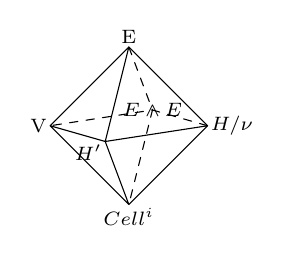
\begin{tikzpicture}[z={(-.3cm,-.2cm)}, % direction z gets projected to; can also change x,y
                                       % use cm to specify non-transformed coordinates
                    line join=round, line cap=round, % makes the corners look nicer
                    every node/.style = {inner sep=1pt, font=\scriptsize}
                   ]
  \draw ( 0,1,0) node[above] {$$} --
        (-1,0,0) node [left] {V} --
        (0,-1,0) node[below] {$Cell^i$} --
        ( 1,0,0) node[right] {$H / \nu$} --
        ( 0,1,0) node[above] {E} --
        ( 0,0,1) node[below left] {$H'$} --
        (0,-1,0) (1,0,0) --
        (0,0,1) -- 
        (-1,0,0) ;
  \draw[dashed] (0,1,0) -- 
  (0,0,-1) node {$E \wedge E$} -- 
  (0,-1,0) (1,0,0) -- 
  (0,0,-1) -- (-1,0,0);
\end{tikzpicture}

The preceding diagram connects the Frobenius structure to differential relations carried by the poincare protocol (of $L_0, L_1)$ which will be used to determine steady state stability and the path integral formulation of open system.
The final step is to define a dual space to the coherence complex $\prod^T_{\Gamma}$ for mapping the functional to the euclidian space.
Each hypergraph category with a so-called dagger functor an involutive contravariant endo functor that is the identity on objects—such that the category is a dagger compact category.
This dagger category corresponds to the complex conjugate of the hilbert space dual which is just its adjoint in the usual sense.
Define $\tau \cong \zeta^{-1}$ (or zeta with arrows reversed) as the conjugate transpose map from dagger category $\zeta^{-1}$, dual to $\zeta$\footnote{https://www.mta.ca/~rrosebru/FMCS2018/Slides/Selinger.pdf}.
Then we have:
\begin{equation}
\int \langle \zeta | \tau \rangle = \aleph_{\zeta, \tau}
\end{equation}
where $\aleph_{\zeta, \tau}$ is the torsor or "constant" geometric relationships to a total volume.
As is clear, all deformations are described in terms of $\aleph_{\zeta, \tau}$.
Kirkov's current law is specified categorically as\footnote{proposition 3.2 https://ncatlab.org/johnbaez/show/Circuit+theory}
\begin{equation}
d^{\dagger} d\phi = i\chi | \chi = rJ
\end{equation}
where the laplacian $\mathcal{L}$ is given by
\begin{equation}
d^{\dagger} d: C^0(\Gamma) \rightarrow C^0(\Gamma)
\end{equation}
is a version of Laplace’s equation with boundary conditions. 
It says the Laplacian of the potential  $\phi \in C^0(\Gamma)$ equals zero except on the boundary of $\Gamma$, where it equals $\chi$.
This is solved like an ordinary differential form: since this function is smooth, we must have $P'(0)=0)$ = 0, $P(t) = \langle d\phi , d\phi \rangle + 2t(\langle d\phi , d\alpha \rangle = 0) + t^2 \langle d\alpha , d\alpha \rangle$ thus
\begin{equation}
P(t) = \langle d\phi , d\phi \rangle + t^2 \langle d\alpha , d\alpha \rangle
\end{equation}
The potential $\phi$ that minimizes the power for a fixed value of $\psi = p \phi$ is a discrete version of the Dirichlet problem.
In the case of the coherence-translation complex, $\langle \zeta | \tau \rangle: C^0(\Gamma) \rightarrow C^0(\Gamma)$ the solution to the dirichlet problem is as follows:
Consider for any $\phi \in C^0(\partial \Gamma)$
\begin{equation}
Q(\psi) = \frac{1}{2} \underset{\phi: p\phi = \psi}{inf} \langle d\phi , d\phi \rangle
\end{equation}
where $\langle d\phi , d\phi \rangle$ defines a nonnegative quadratic form on the finite-dimensional vector space $C^0(\Gamma)$ and the constraint $\phi = \psi$ picks out a linear subspace of this subspace.
Its derivative defines an element of the dual space $C_0 (\partial \Gamma)$ denoted by $dQ_{\tau}$ this element is equal to the boundary current J corresponding to the boundary voltage $\tau$ such that $dQ_{\tau} = J$.
Given a linear operator $f: C^0(\partial \Gamma) \rightarrow C^0(\Gamma)$, define the Fiber-current $I_F = \lambda^{-1}p = \alpha^{-1}$ and boundary current $J_\alpha = \lambda \alpha(\lambda, p) = \lambda^2 / $, for any $\tau' \in C^0(\partial \Gamma)$ the power can formulated in terms of a dirichlet form as follows
\begin{equation}
Q(\tau) = \sum_{i, j} c_{i, j}(\tau_i - \tau_j)^2
\end{equation}
\end{proof}

It follows that $Cell \cong \blacksquare$ in terms of the solution its Dirichlet problem.

\subsubsection{Utility Theory of Arbitrage Free Networks}
By the Topological Second Law of Thermodynamics and Entropy Rate and $\mathcal{\chi}_T$ can only increase or stay constant with t.
Thus we can calculate the Utility of $\Omega \in ConTop$ using the efficiency of real heat engines.
Consider the Carnot engine, which can be hooked in series and the composite efficiency debit is the product of individual debits.
Between two information reservoirs, all Carnot engines have the same efficiency and thus the same efficiency debit, otherwise it would be possible to create a "heat arbitrage" creating a "perpetual motion machine of the second kind."
The composite efficiency debits between any two reservoirs implies path independence.
Thus by Ellerman's arbitrage theorem, the second law implies that there exists $m+1$ positive real "prices" $T_0 \dots T_m$ such that for any Carnot engine operating between nodes h and c, the efficiency debit is $r = \frac{T_c}{T_h}$.
Define a thermodynamic engine defined by Ellerman's arbitrage theorem an Economic Engine.

\begin{theorem}
Efficiency of the Economic Engine is equivalent to the efficiency of an electrical circuit.
\end{theorem}

\begin{proof}
If the "prices" are normalized so that the freezing and boiling points of water differ by 100 units, then the "prices" are the Kelvin Absolute Temperatures of the reservoirs.

Thus we can describe the efficiency of ConTop or its component protocols as
\begin{equation}
e = 1 - (\frac{dQ_c}{dQ_h})
\end{equation}
and the efficiency debit as $r = 1 - e = \frac{dQ_c}{dQ_h}$.
It follows from the definition of the extended power functional for the ConTop that the efficiency (MWe\footnote{https://energyeducation.ca/encyclopedia/Megawattselectric}) for output $o \cong c$ and input $i \cong h$ is given by
\begin{equation}
e = \frac{dQ_o}{dQ_i}
\end{equation}
\end{proof}

\begin{theorem}
For a ConTop Complex, as Cells of higher rank eclipse Cells of lower rank, or as the coboundary that is the bounded colimit of an open system grows relative to $\Omega_0$, the overall efficiency increases.
\end{theorem}

\begin{proof}
In order to understand efficiency of Cell complex, we need to extend the definition of utility for circuits into an information theoretic complex, namely the Minimum free energy complex.
The total free energy is a Kullback-Leibler divergence and a special case (symmetric in the interacting body) of the free energy introduced by Baez and Pollard\footnote{Baez, J.; Pollard, S. Relative Entropy in Biological Systems. Entropy}.
A general information structure is defined by the triple $(\Omega, \prod, P)$ above which can be used to form a simplicial information cohomology complex which can be triangulated like space-time representations such as causal sets; this was actually alluded to via Blockchain Cohomology as the equivalence of $\Omega$ with Sorkin's Fintoposets.
For our minimum free energy complex $(\Omega, \prod, P)$, the finite information rate r of an information path is
\begin{equation}
r = lim \frac{H_k}{k}
\end{equation}
(the evolution of entropy $H_k$ when the number of variables k increases).
By noting the equivalence of the io black box functor and the category of circuits which carries the extended power functional
\begin{equation}
e = \frac{dQ_o}{dQ_i} = \frac{\Omega - \Omega_0}{\Omega_0} \underset{\lim{\Omega >> \Omega_0}}{\mapsto} \frac{\Omega}{\Omega_0} - 1
\end{equation}
and can be seen as an increase in the latent variables contained in the coboundary $H_k$ (ways in which they can mix or nonlinear effects) as the number of variables in the base layer $\Omega_0 = k$ increases.
It follows that as more consuming channels in ConTop eclipse producing, that is as the coboundary that is the bounded colimit of an open system grows relative to $\Omega_0$, the overall efficiency increases.
This is an artifact of the fact that as more producers become consumers of other producers, there is an increase in cross information and thus Kulbak-Leibler (KL) divergence increases. 
\end{proof}

\subsection{Equilibria Analysis}
Now we can define the Pareto optima for ConTop.
The definition of boot vector of Ellerman's boot system can be extended via the triangulated category and in terms of spiders along the enrichment.
This will give a 1:1 formulation of the matrix calculus for the Lagrangian multipliers in terms of signal flow graphs.

\begin{theorem}
For ConTop complexes, the solution spectra for utility function equilibria are given by the Cheeger bounds of the manifold.
\end{theorem}

\begin{proof}
Utility maximization implies that the market must be arbitrage free, which is described as
\begin{equation}
\frac{MU_1}{p_1} = \frac{MU_2}{p_2} \dots = \frac{MU_n}{p_n}
\end{equation}
"Markets" or market graphs can be defined in terms of the marginal data $F(\hat{x})$ and $\nabla f^0 (\hat{x})$.
If $(\hat{x})$ is feasable, regular and a local maximum, then any market graph defined from marginal data $\nabla f^0 (\hat{x})$ and $-F(\hat{x})$ must be arbitrage-free. There is a vector $P = (1, p_1 \dots p_m)$ of normalized cofactors which is a price vector for any such market graph and the normalized cofactors $p_1 \dots p_m$ are the lagrange multipliers associated with the m constraints.
The market is only arbitrage-free if and only if the n transformation rates $\frac{f_i}{g_i} \dots \frac{f_n}{g_n} = \mu$ where the common rate of transformation is the Lagrange multiplier $\mu$. 
Let the matrix A
$\begin{pmatrix}
f_1 & \dots & f_n\\
g_1 & \dots & g_n
\end{pmatrix}$
where -g i is used instead of + g, since $g(x_1 \dots x_n)$ represents the amount of the resource used-up.  Consider  any  column of this market matrix  coupled with the  dummy column to form a  square matrix:
$\begin{pmatrix}
? & f_i\\
? & -g_i
\end{pmatrix}$
The cofactors of the  dummy column are the local  prices $P_y = - g_i$ and $P_b = - f_i$ so (assuming $g_i \neq 0$) the price  of b in terms of the  numeraire y is the  transformation  rate 
\begin{equation}
b \xrightarrow{P_b/P_y = f_i/g_i} y
\end{equation}
defined by the marginal  variations in the instrument  $x_i$.
Consider the matrix of partials of the constraints evaluated at the candidate point $x^0$, G:
$\begin{pmatrix}
g^{1}_1 & \dots & g^{1}_n\\
\dots & \dots & \dots \\
g^{m}_1 & \dots & g^{m}_n
\end{pmatrix}$
For the  intuitive  market to be arbitrage-free, all the local cofactor prices $(P;, Pb,, Pb2)$ defined by any set of $m >= 2$ instruments must be scalar  multiples of the  non-zero price vector $(P,, Pb,, PbJ. $ In  formal terms,  the market matrix defined by the  problem is
$\begin{pmatrix}
\nabla f\\
- G
\end{pmatrix}$
The candidate point $x^0$, satisfies the  constraints and is regular in the sense that the $M \times m$ matrix $G[g^j_i]$ is of full low rank.
It follows that there are m columns forming a non-singular submatrix $G^*$. 
If $f^*$ is th evector fo the corresponding m partials of $f$ then consider the $(m + 1) \times (m + 1)$ matrix:
$\begin{pmatrix}
? & f^*\\
? & -G*
\end{pmatrix}$
where the cofactors of the  dummy column  form the local cofactor prices $P_y, P_{b_1} \dots P_{b_m}$determined by the m chosen instruments.
The intuitive market is arbitrage-free if all the $C(m, n)$ vectors of local cofactor prices are scalar multiples  of this  non-zero  vector.
In formal terms, the first order necessary condition for   the   candidate point xo to be a  constrained  maximum is equivalent to the condition that the market matrix of the problem A = 
$\begin{pmatrix}
\nabla f\\
- G
\end{pmatrix}$
is arbitrage-free which, stated  in the  Arbitrage in turn, is equivalent to the other conditions Theorem for  Market Matrices.

Consider the equivalent market matrix formed from ConTop
$\begin{pmatrix}
\prod^T_\Gamma \\
- H
\end{pmatrix}$
and note the signature of its matrix as the copy generator\footnote{https://graphicallinearalgebra.net/2015/06/09/matrices-diagrammatically/}
% https://q.uiver.app/?q=WzAsMjUsWzMsMiwibSJdLFs3LDBdLFswLDFdLFswLDNdLFs1LDFdLFs1LDNdLFs3LDFdLFs3LDNdLFsxMywzXSxbMTMsMV0sWzEsMiwiXFx0aGV0YSJdLFsyLDFdLFsyLDNdLFs1LDBdLFsyLDBdLFsyLDRdLFs1LDRdLFsyLDJdLFs3LDIsIj0iXSxbOSwzXSxbMTAsMSwiSV9tIl0sWzEwLDIsIklfbSJdLFsxMSwzXSxbOSwwXSxbMTEsMF0sWzAsNCwiIiwwLHsiY3VydmUiOi0xLCJzdHlsZSI6eyJoZWFkIjp7Im5hbWUiOiJub25lIn19fV0sWzAsNSwiIiwwLHsiY3VydmUiOjEsInN0eWxlIjp7ImhlYWQiOnsibmFtZSI6Im5vbmUifX19XSxbMTQsMTUsIiIsMix7ImN1cnZlIjoyLCJzdHlsZSI6eyJoZWFkIjp7Im5hbWUiOiJub25lIn19fV0sWzEzLDE2LCIiLDEseyJjdXJ2ZSI6LTMsInN0eWxlIjp7ImhlYWQiOnsibmFtZSI6Im5vbmUifX19XSxbMCwxNywiIiwyLHsic3R5bGUiOnsiaGVhZCI6eyJuYW1lIjoibm9uZSJ9fX1dLFsyMywxOSwiIiwyLHsiY3VydmUiOjMsInN0eWxlIjp7ImhlYWQiOnsibmFtZSI6Im5vbmUifX19XSxbMjIsMjQsIiIsMix7ImN1cnZlIjozLCJzdHlsZSI6eyJoZWFkIjp7Im5hbWUiOiJub25lIn19fV1d
\[\begin{tikzcd}
	&& {} &&& {} && {} && {} && {} \\
	{} && {} &&& {} && {} &&& {I_m} &&& {} \\
	& {\theta} & {} & {m} &&&& {=} &&& {I_m} \\
	{} && {} &&& {} && {} && {} && {} && {} \\
	&& {} &&& {}
	\arrow[from=3-4, to=2-6, curve={height=-6pt}, no head]
	\arrow[from=3-4, to=4-6, curve={height=6pt}, no head]
	\arrow[from=1-3, to=5-3, curve={height=12pt}, no head]
	\arrow[from=1-6, to=5-6, curve={height=-18pt}, no head]
	\arrow[from=3-4, to=3-3, no head]
	\arrow[from=1-10, to=4-10, curve={height=18pt}, no head]
	\arrow[from=4-12, to=1-12, curve={height=18pt}, no head]
\end{tikzcd}\]
$ \theta \mapsto \begin{pmatrix}
1 \\
1
\end{pmatrix}: 1 \rightarrow 2$
which clearly maps to the spider diagram of the open bound colimit.
The GraphCospan H admits decomposition into a flattened matrix of partials by the definition of the lagrangian.
These partials define the steady state equilibria of a Price Index across all $\epsilon$ sheaf types carried by the Cell complex.

As a final step, let's re-formulate the calculation of Efficiency above in terms of the in and out degree of each Cell.
By definition of the Cell Lagrangian, it forms a linear subspace which implies the existence of linear relations\footnote{https://graphicallinearalgebra.net/2015/12/26/27-linear-relations/}.
Thus, we can construct a linear relation out of the Dagger category as it is always the weak inverse of R. and enforce that for any Cell diagram we have
\begin{equation}
d * d^{\dagger} * d = d
\end{equation}
which means that the volume of d does not fluxuate, or is a normalized linear relation.
By symmetry, this dagger category is given by the $m$-discard generator, which is the m zero generators direct summed together yielding the following linear relation $ \theta \mapsto \begin{pmatrix}
I_m \times I_m & I_m \times I_m \\
I_m \times I_m & I_m \times I_m
\end{pmatrix}$
and a generator of Rel as the dimensions of the matrix $m \times n$ is given by the open coboundary of open systems.
By the "special" equation\footnote{https://graphicallinearalgebra.net/2015/09/08/21-functions-and-relations-diagrammatically/} implies that $2=1$ which is true in the case of when composing relations, which keeps track of paths (just as the natural number matrices), it’s just that we are only interested in the Yes or No question “Is there a path?”, and we don’t care about the number. 
This is one interpretation of (S): it ensures that having 100 paths is the same as having 1 path (but different to no paths).

By using this fact of Rel, we can redefine utility in terms of the dagger-hypergraph category and wiring functions of the dot-diagram of GraphCospan\footnote{https://arxiv.org/pdf/1406.5942.pdf}
\begin{equation}
e = \frac{dQ_o}{dQ_i} \underset{\lim{\Omega >> \Omega_0}}{\mapsto} \frac{\Omega}{\Omega_0} - 1 \implies \frac{\Omega}{\Omega_0} \in \{0 \dots 2\}
\end{equation}
\begin{equation}
r = 1+e = \frac{dQ_o- dQ_i}{dQ_i} = \frac{|A - G|}{A}
\end{equation}
which equals 0 if optimal.
Note this is an equivalent definition of the coherence complex but incorporating state metadata into the creation of H.
The solution spectra to s Cell is given by the varaince bounding of the Cheeger bounds\footnote{https://www.maths.lancs.ac.uk/~sherlocc/ResearchTutorials/L2var.pdf}, which are given by the co/homological dimensions of the manifold of a given Cell sub-complex in the total complex ConTop.
\end{proof}

\subsubsection{Pareto Optima}
We can now define Pareto optima for ConTop and the coherence complex.
Consider a Pareto Allocation as Pareto optimal or Pareto efficient\footnote{https://are.berkeley.edu/~traeger/Lectures/ClimateChangeEconomics/Slides/}, if it is not possible to reallocate the resources of the economy in a way such that possible to reallocate the resources of the economy in a way such that at least one person is better off without making any other person worse off.
In a competitive economy, all firms maximize profits, individuals maximize their utility and markets clear.
A competitive economy's market equilibrium is defined by the Pareto optimal steady states of its utility curves.
It follows that a competitive economy is the goal of generative economics, thus we can show the success of our construction ConTop and concretely define the steady state solutions of a Pareto optimizing consensus protocol.

Consider the 'attainable states' $W$ as a subset of a 'commodity space' $P^m$, an open set in the Cartesian space $R^l$.
Define
\begin{equation}
W = \{ x \in P^m | \sum x_i = w \}
\end{equation}
an open subset of an affine subspace with compact closure in $(R^l)^m$.
Each consumer is supposed to have his preferences represented by a function $u_i:P \rightarrow R$, their utility function which we suppose as differentiable as necessary.
Thus consumer i prefers $x'_i$, to $x_i$ if and only if $ui(x',)> ui(xi)$. 
Consumer $i$ is indifferent to commodity bundles in the same level surface of $u_i$.
Hence the  $u^{-1}_i(c)$ are called indifference surfaces. 

let $\pi_i: P^m \rightarrow P$ be the projection $\pi_i(x) = x_i$ then the we have induced functions on W, still denoted by  $u_i$, defined as the composition 
\begin{equation}
W \xrightarrow{inclusion} P^m \rightarrow P \xrightarrow{u_i} R
\end{equation}
One considers exchanges in W, which will increase the utility of each consumer or increase each $u_i$ on W.
A state $x \in W$ is called Pareto optimal if it has the property; there is no $x' \in W$ with $u_i(x') \geq u_i(x)$, all i, and $u_j(x') > u_j(x)$, some j. 
The idea is that if $x \in W$ is not Pareto, then it is not economically stable.

In the abstract setting of Smale's Pareto theory\footnote{https://sci-hub.se/https://www.sciencedirect.com/science/article/abs/pii/0304406874900020} the idea of the following 'Hessian'\footnote{https://sci-hub.se/https://link.springer.com/article/10.1007/BF00485983} is to obtain a criterion for a point $x \in W$ to be a stable Pareto point.
The Hessian $H_x$ for utility $u: W \rightarrow R^m$ at $x \in \theta$, where u is $C^r$ and x satisfies the rank condition, is negative definite.
If u satisfies the "transversality condition" (given by the Fredholm operators of + and - \footnote{Corollary B.14, Generic Morse–Smale property for the parabolic equationon the circle}) and has no cycles, gradient vector field for u is a smooth tangent vector field X defined over W with the property that $X(x)\in H(x)$ for $x \notin \theta$ and $X(x)=0$ for $x \in \theta$ which corresponds to morse relations given by
\begin{equation}
M_i = \sum_{\lambda} dim H_{i - \lambda}(\theta_{\lambda}, \theta_{\lambda}')
\end{equation}
where $\theta_{lambda}$ is the set of $x \in \theta$ with index $\lambda$ and nullity zero and $\theta_{n}$ the set of $x \in \theta$ with nullity positive.
The coefficients of $M_i$ are given by an arbitrary field and specializes to $m=2$ 
\begin{equation}
M_m = dim H_1(\theta_{n - 1}, \theta_{n - 1}')
\end{equation}
however m can be extended beyond two to create an m-dimensional ETF or collateralized swap, which will be shown below.

\begin{theorem}
Commodities defined as the composition of ConTop complexes obey global enrichment.
\end{theorem}

\begin{proof}
A dynamical system is a gradient system on $X, \dot{x} = f(x)$ if there is some function $V: X \rightarrow R$ such that $f(x) \equiv -D V(x)$.
The function $V(x)$ is often referred to as the potential function of the system; $f(x)$ is called the gradient of V at x.
The directional derivative of V(x) in the direction $h=(h l \dots hn), \rVert h \rVert  = 1$, is defined to be $DV(x) \dot h$. 
The directional  derivative measures how fast the function V is increasing in the direction h; as the above formula indicates, it is just the projection of $DV(x)$ on the vector h. 
It is therefore clear that this projection will be maximized  when DV(x) itself points in the direction h.
Thus we have a  nice geometrical interpretation of the gradient: it points in the direction where V increases most rapidly.

The primary feature of Hamiltonian systems (of which the above hessian is an example) for economic applications is that they have certain desirable stability properties.
In the classical theory of Hamiltonian mechanics, H was quadratic so that the Hamiltonian system was a  linear system of differential equations.
In this case a classical theorem of Poincare shows that if X is an eigenvalue of the linear system at $(x^*, y^*)$ then $-X$ is also an eigenvalue.
Thus the equilibrium of the Hamiltonian system are symmetric saddle points.
In the general case, where the Hamiltonian is nonlinear, the same kind of saddle point property occurs when the function is concave in x and convex in y. 

The Lyapunov exponents correspond to the original price index matrix's steady states where it is defined across the tensor and not just the direct sum.
This enforces braiding and allows a flattened Pareto optima matrix.
Note: this flattened matrix is actually given by the diffusion map below, which can be formed due to the conjugate dual definition of A.
The commodities in composed protocols correspond to "ETFs" or synthetic financial products constructed out of the configuration of many states in a certain order following the global enrichment.
\end{proof}

\subsection{Transition Matrices for ConTop}
Dynamical systems where stability is of concern are often described in terms of Ergodicity, or the tendency for a system state to always return to a starting mode.
Up until this point we have extended the the locally unstable globally stable Morse Smale systems with the ordinary poincare metric and extended this (trivially) with the Fisher information metric.
This connects the nerve/atlas space for Gibbs Microcanonical Partition Functions of Entropic forces\footnote{34  https://www.mdpi.com/1099-4300/18/8/309/htm} to the theory of Entropic forces as $\partial \mathbb{Nu}$ has units of inverse of energy and corresponds the locally unstable manifold.
Both manifolds are then bound by the Freedholm equation ($g(t)$, 125), which is essentially just the coherence complex defined cohomologically.
In turn the Freedholm formulation is connected to the theory of Entropic forces, as we will show bellow.
First, a closed form Markov Partition and matrix transition formulation of ConTop is formed for computational refinement.

\subsubsection{Transition Matrix for ConTop with n-state channels}
Consensus probability can be formed in terms of opinion formation which is a prototypical class of markov process on a network\footnote{5.7 https://arxiv.org/pdf/1612.03281.pdf}.
The probability of consensus or convergence of the protocol complex can be defined in terms of the DeGroot model by imposing a conservation of opinions where $\sum^N_{i=1} F^{DG, disc}_i x_i (n)$ is  conserved  over  time  for  positive  constants $F^{DG, disc}_i$ (with $i \in 1\dots N)$ where  the  superscript  “disc”  stands  for  discrete  time  and $ \sum^N_{i=1} F^{DG, disc}_i = 1$.
This implies that $F^{DG, disc}_i$ quantifies the influence of $v_i$ on the final opinion in consensus. 

\begin{theorem}
The functional probability of convergence of a consensus network $F^{ED}_i$ is isomorphic to the utility of a thermo-electric system, namely 
$F^{ED}_i = (const) \times \frac{s^{out}_in}{s^{in}_{out}}$
\end{theorem} 

\begin{proof}
By imposing this conservation law, one obtains
\begin{equation}
\sum^N_{i=1} F^{DG, disc}_i x_i (n - 1) = \sum^N_{i=1} F^{DG, disc}_i x_i (n) = \sum^N_{i=1} F^{DG, disc}_i x_i (n) ( \sum^N_{i=1} A_{ji} x_j (n-1) )
\end{equation}
by requiring that the above holds for $ (with x_i(n-1)i \in 1\dots N $ 
\begin{equation}
F^{DG, disc}_i  = \sum^N_{i=1} A_{ji} F^{DG, disc}_j
\end{equation}
where $F^{DG, disc}_i $ is the stationary density of a DTRW (discrete time random walk) and whose transition-probability matrix is  $A^{\intercal}$ the  adjacency  matrix  of  the  edge-reversed  network $D^{rev}$.

For the continuous case of node influence metrics $x$ we have 
\begin{equation}
\frac{d x(t)}{dt} = (A^{\intercal} - D^{rev}) \equiv -L^{rev} x(t)
\end{equation}
where $D^{rev}$ is the diaagonal matrix whos $(i, i)$th element equals $s^{in}_{out}$ and $L^{rev} $ is the combinatorial Laplacian matrix for the edge-reversed network.
The left eigenvector of $L^{rev}$corresponding  to  eigenvalue  0  gives  the  station-ary  density  of  the  Poissonian  edge-centric  CTRW  on  the  edge-reversed  net-work. 
The  corresponding  right  eigenvector  gives  the  asymptotic  state  of  the continuous-time  DeGroot  model. 
This also has an interpretation as linear synchronization dynamics that results from linearizing nonlinear systems such as Dirichlet forms above.

Thus for $L_0$ consensus occurring linearly across the free dimension of the enrichment $n \in 1 \dots + \infty \subseteq \mathcal{N}$, define the vector form of the dynamics as the following recurrent matrix equation
\begin{equation}
x(n) = A^{\intercal} x(n-1)
\end{equation}
where $x(n) = (x_1(n), \dots, x_N (n))^{\intercal}$ are the opinions or proposals of all proposing nodes $v \in v_i$.
The  initial  opinion $x_i(0)$  of  the final opinion $O: x^{*}_1 = \dots = x^{*}_N$ of consensus.
If $O$ is close to $x_i(0)$ one  interprets  node $v_i$ as being influential.
If such a conserved quantity exists, one obtains
\begin{equation}
O = \sum^N_{i=1} F^{DG, disc}_i x_i (0) = \sum^N_{i=1} F^{DG, disc}_i x^{*}_i = x^{*}_1 = \dots = x^{*}_N
\end{equation}
If we consider the observation to follow a poisson distribution (such as the poisson-dirichlet form) then for observations given by poisson process $p(t)$ with edge rate $N A_{i, j} / \sum^N_{i', j' = 1} A_{i', j'}$ and  an  event  induces  a local consensus event (equivalently to opinion dynamics) for a single random walker the master equation it satisfies is 
\begin{equation}
\frac{d p(t)}{dt} = p(t)(A^{\intercal} - D^{rev}) \equiv -P(t)L^{rev}
\end{equation}
Then the consensus probability  $F^{ED}_i$ for each node is given by the equilibrium of $\frac{d p(t)}{dt}$.
That is
equation it satisfies is 
\begin{equation}
(F^{ED}_1 \dots F^{ED}_n)L^{rev} = 0
\end{equation}
We can obtain an intuitive understanding of above by writing a recursive equation for the consensus probability when the process starts from a single node $v_i$ with opinion 0 (i.e., for $F^{ED}_i$).
We obtain
\begin{equation}
F^{ED}_i = \frac{A_{i, j}}{\sum^N_{j'=1} A{i', j'}} + \frac{\sum^N_{j=1} A{j, i}}{\sum^N_{j'=1} A{i', j'}} \times 0 + \frac{\sum^N_{i', j'=1; i'=i; j'=j} A{i', j'}}{\sum^N_{i', j'=1} A{i', j'}}
\end{equation}
where $F^{ED}_{i,j} = F^{ED}_i + F^{ED}_j$ is the probability that one reaches the consensus of opinion 0 start-ing from the configuration in which $v_i$ and $v_j$ but no other nodes have opinion 0.
Thus we have our functional probability of convergence given by
\begin{equation}
\sum A_{i,j} F^{ED}_j = F^{ED}_j \sum A_{ji} = (F^{ED}_1 \dots F^{ED}_n)L^{rev} = 0
\end{equation}
If  the  network  is  directed,  we  obtain  a  first-order  approximation  to the consensus probability of a node by applying Eq81\footnote{https://arxiv.org/pdf/1612.03281.pdf}
\begin{equation}
F^{ED}_i = (const) \times \frac{s^{out}_in}{s^{in}_{out}}
\end{equation}
which is isomorphic to the calculation of utility based on efficiency of a thermoelectric system.
\end{proof}

\subsubsection{Transition Matrix for ConTop $L_0$ and Forgery Probability}
The transition-probability  matrix $T$ has  elements $T_{ij}$,  which  give  the  probability that a walker (state of network) moves from $v_i$ to $v_j$, of
\begin{equation}
T_{i, j} = \frac{A_{ij}}{s^{out}_{in}} | s^{out}_{in} > 0
\end{equation}
and $\sum T_{i, j} = 1$, for the largest eigenvalue $\lambda_l \leq 1$ for directed graphs such as ConTop.
This  transform,  called  the“graph  Fourier  transform”,  generalizes  the  standard  Fourier  transform  of  an RW  [see  Eqs.  (3)  and  (7)],  and  the  eigenvectors  of  the  transition-probability matrix T play the role of the Fourier modes.

\begin{theorem}
For a transition-probability  matrix $T$ representing consensus, the Exit Probability can be used to determine the criteria for Forgery, or an invalid state in $L_0$.

\end{theorem}

\begin{proof}
The transition-probability matrix T then has the following form
\begin{equation}
T = 
\begin{pmatrix}
Q && R  \\
0 && \mathcal{I}
\end{pmatrix}
\end{equation}
where $Q$ is an $N_1 \times N_1$ matrix that describes transitions between transient-statenodes, $R$ is an $N_1 \times N_2$ matrix that describes transitions from transient-state nodes  to  absorbing-state  nodes,  and $I$ is  the$ N_2 \times N_2$ identity  matrix  that corresponds  to  individual  absorbing-state  nodes.
Taking powers of T yields
\begin{equation}
T^n = 
\begin{pmatrix}
Q^n && R(\mathcal{I} + Q \dots Q^{n-1})  \\
0 && \mathcal{I}
\end{pmatrix}
\end{equation}

Suppose that we start from transient-state node vi and want to calculate the mean number of visits to transient-state nodevjbefore reaching an absorbing-state node
This number of visits is equal to the (i,j)th element of the matrix
\begin{equation}
W = \sum^{\infty}_{n=0} Q^n = (I - Q)^{-1}
\end{equation}
because  the  (i,j)th  element  ofQnis  equal  to  the  probability  that  a  randomwalker starting from vi vis its v jat discrete time n.
The matrixWis called the“fundamental matrix” associated withQ. 
The matrix on the right-hand side of $W$ s called the “resolvent” ofQ. 
Similar considerations arise in the study of “central” (i.e., important) nodes in networks as described above.
The “exit probability” (i.e., the “first-passage-time probability”) is defined as the probability Uij that the walker terminates at an absorbing state vj when it  starts  from  a  transient  state vi.  
When  there  are  multiple  absorbing-statenodes, it is nontrivial to determine the exit probability. 
The probability that the walker reaches vj after exactly n steps is given by the (i,j)th element of $Q^{n-1}R$. 
Therefore, we obtain the exit probability in matrix form as follows:
\begin{equation}
U = \sum^{\infty}_{n=0} Q^{n-1} = W R
\end{equation}
\end{proof}

Thus we can determine the time limit for convergence in terms of $\aleph$ as the exit probability for $v -3$ byzantine nodes and $v-1$.
If $p(\aleph(t)) < \frac{\lVert (U(v_b - v)) \rVert }{\lVert (U(v)) \rVert}$
 then for byantine nodes $(v_b)$ then the error bounds are
\begin{equation}
\lVert (U(v)) \rVert  \times p(\aleph(t)) > \lVert (U(v_b - v)) \rVert
\end{equation}
which means that the time to make one proposal must be bound by the time taken to make all proposals made by the computational complexity of $\aleph$.

Thus, for $L_0$ at any point each node creates a probability distribution based on a special type of random walk called a self avoiding walk which comprises the entries of of $A^{\intercal}$ that is normalized across all $v_r$ such that $\sum^r_{j=1} = 1$. 
For $L_0$ the value $s^{out}_{in}$ is given by the seeder/leecher ratios of states reserving each other's thoughput.
Thus we have
\begin{equation}
T(v) = \frac{1}{\sqrt{s_v}} A^{\intercal} S_{v} 
\end{equation}

\subsection{Cellular Reserve Banking}
Finally, we can define the roll of a protocol in arbitrating resources and economic stability. 
Each Cell and Cell complex within ConTop can be equipped with its own relative interest rate.
This is moreso a fact of a topos, for which exponentiation relative to its own domain and global domain is possible. 
Because of this, consensus protocols can act as their own arbitrating authority in defining financial policy.
For a decentralized network this translates from interest rate fluctuation and injection of capital into a particular sector, into fluctuations of validator rewards and resources offered.
However, as will be shown, there is a distinct difference between a Generative Economy and centralized Capitalism: resources or needs of each individual Cell or complex in the economy can be met while still maintaining an invariant of no arbitrage.
For any agent to act freely in an economy and the policymaker of a Central Bank violates the definition of no arbitrage in that they are privy to more information about the global economy than the average individual agent or firm.
ConTop complexes, as the arbitrators of a currency, can perform the same role as Central Banks while still enforcing the law of no arbitrage.
Define the Cellular Reserve Bank as the optimization of a loss function parameterized by Output Gap or and an aggregate measure of (computational) resource strain in the economy and inflation.

\begin{lemma}
A coherence complex's surface of least action simplifies to the traditional Central Bank shock response curve.
\end{lemma}

\begin{proof}
First consider the path integral formulation of the coherence complex.
\begin{equation}
\int \langle \zeta | \tau \rangle = U(x_1 \dots X_n; P_N)  - \sum_{t(e)=n} I(e)) + (\sum_{t(e)=n} I(e) -G(x_1 \dots X_n; P_N))
\end{equation}
Where the potential and kinetic energy is both fitted according to the current $I$ which encodes the flow of actions of actual state space vs the ideal state space.
If we optimize with respect to mean square error between predicted and actual state matrices we have
\begin{equation}
\langle \zeta | \tau \rangle = (U(x_1 \dots X_n; P_N) - U(I(e)))^{2}  + (G(i(e)) -G(x_1 \dots X_n; P_N))^{2}
\end{equation}
which is a discrete manifold that describes a surface on the differential form of this particular coherence complex.
This is the full solution spectrum to the validation of state hierarchically through the hypergraph surfaces of each rank in the poincare protocol complex.
If we reduce the dimensionality strictly to the terminal object, or protocols of complexity $L0$, the dimensions of relative (by some linear factor $\beta$) minting rate $m$ and a fixed production rate $p$ we have 
\begin{equation}
\langle \zeta | \tau \rangle_0 = \beta (m_0 - m)^{2}  + (p_0 - p)^{2}
\end{equation}

If we further parameterize such that we substitute with the Phillips curve
\begin{equation}
m_0 = m + \alpha (p_0 - p)
\end{equation}
we have 

\begin{equation}
\langle \zeta | \tau \rangle_0 = \beta (m + \alpha (p_0 - p) - m)^{2}  + (p_0 - p)^{2}
\end{equation}
differentiating we have
\begin{equation}
\nabla_p \langle \zeta | \tau \rangle_0 = \alpha \beta (m + \alpha (p_0 - p) - m) + (p_0 - p) = 0
\end{equation}
giving
\begin{equation}
\nabla_p \langle \zeta | \tau \rangle_0 = \alpha \beta (m0 - m) + (p_0 - p) = 0
\end{equation}
and
\begin{equation}
\alpha \beta (m0 - m) = (p_0 - p)
\end{equation}
which is precisely the Central Bank utility loss function.
\end{proof}

It can now be shown that ConTop complexes will always be more efficient than Central Banks with regards to utility via arbitrage reduction.

\begin{theorem}
ConTop complexes of rank $\geq$ = 1 are more efficient than L0 utility loss.
\end{theorem}

\begin{proof}
Consider the efficiency of an economic engine
\begin{equation}
e = \frac{dQ_o}{dQ_i} = \frac{\Omega - \Omega_0}{\Omega_0} \underset{\lim{\Omega >> \Omega_0}}{\mapsto} \frac{\Omega}{\Omega_0} - 1
\end{equation}
As has been shown in the preceding lemma, utility optimization for Central Banks is the linearization of ConTop, i.e. first order approximation.
Thus Central Bank policies will always be bounded by the higher order terms of ConTop complexes, which means that
\begin{equation}
\frac{\Omega}{\Omega_0} << \frac{\langle \zeta | \tau \rangle}{\Omega_0}
\end{equation}
where $\langle \zeta | \tau \rangle$ is the full sollution spectrum of the given complex and $\Omega$ is its first order rank system.
\end{proof}
Thus we have shown that any system with increasing complexity or rather with globally converged information gain will always eclipse centralized policies.

\section{Conclusion}
A new calculus of generative effects was introduced and used to derive the Economic Theory of Generativity. 
From the Economic Theory of Generativity the Economic Engine was defined and used to compare Central Reserve Banking vs Cellular Reserve Banking.
Key takeways are that the Generative Calculus can be extended to the wider field of generative effects.
And that Cellular Reserve banking is promising a evolution of the arbitrage-riddled global banking system that maintains stable utility.


\bibliographystyle{plain}
\begin{thebibliography}{9}
\bibitem{latexcompanion} 
Baez, John C
\textit{Circuitry, EE and chain complexes}.
\\\texttt{https://math.ucr.edu/home/baez/week288.html}


\bibitem{latexcompanion} 
Baez, John C
\textit{Physics, Topology, Logic and Computation:A Rosetta Stone}.
\\\texttt{https://arxiv.org/pdf/0903.0340.pdf}

\bibitem{latexcompanion} 
PIETER HOFSTRA AND PHILIP SCOTT
\textit{ASPECTS OF CATEGORICAL RECURSION THEORY}.
\\\texttt{https://arxiv.org/pdf/2001.05778.pdf}

\bibitem{latexcompanion} 
David Spivak, Brendan Fong
\textit{Seven Sketches in Compositionality}.
\\\texttt{https://math.mit.edu/~dspivak/teaching/sp18/7Sketches.pdf}

\bibitem{latexcompanion} 
Pierre Baudot
\textit{The Poincaré-Shannon Machine: Statistical Physics and Machine Learning Aspects of Information Cohomology}.
\\\texttt{https://www.mdpi.com/1099-4300/21/9/881}


\bibitem{latexcompanion} 
Tobias Fritz
\textit{A synthetic approach to Markov kernels, conditionalindependence and theorems on sufficient statistics}.
\\\texttt{https://arxiv.org/pdf/1908.07021.pdf}

\bibitem{latexcompanion} 
Tatsuya Hagino
\textit{A Categorical Programming Language}.
\\\texttt{web.sfc.keio.ac.jp/~hagino/thesis.pdf}

\end{thebibliography}
\end{document}
